\documentclass[twocolumn,letterpaper]{IEEEAerospaceCLS}

\newcommand\hmmax{0}
\newcommand\bmmax{0}

%%%%%%%%%%%%%%%%%%%%%%%%%%%%%%%%%%%%%%%%%%%%%%%%%%%%%%%%%%%%%%%%
% PACKAGES
%%%%%%%%%%%%%%%%%%%%%%%%%%%%%%%%%%%%%%%%%%%%%%%%%%%%%%%%%%%%%%%%

\usepackage{graphicx}
\usepackage{subfig}
\usepackage{epstopdf}
\usepackage{enumitem} 		% easier-to-edit lists
\usepackage[tight]{units} 	% includes nicefrac package
\usepackage{amsmath}		% Needed for align environment
\usepackage{amssymb}		% Needed for \lesssim symbol
%\usepackage{algorithm}		% algorithm-environment
%\usepackage{algpseudocode}  % For \algorithmic
\usepackage{gensymb}		% \degree command
\usepackage{booktabs}  		% Allows layouting nicer tables
\usepackage{multirow}		% Multirows in tables
\usepackage{tikz}			% Tikz-figures
\usetikzlibrary{shapes,arrows,quotes}
\usetikzlibrary{calc}
\usepackage[bottom]{footmisc}		% Load before hyperref to avoid problems
\usepackage[colorlinks=true,citecolor=blue]{hyperref} %Hyperlinks for refs&cites in the PDF
\usepackage{mathtools}		% \coloneq (define as equal to) operator and more
\usepackage{bm}				% For \bm
\usepackage[capitalize,noabbrev]{cleveref} % CleverRefs ; Must come last
\usepackage[nolist,nohyperlinks]{acronym}
\usepackage{array}
%\usepackage{pseudocode}  	% For \pseudocode

\crefname{equation}{Eq.}{Eqs.}
\Crefname{equation}{Equation}{Equations}
\crefname{appsec}{Appendix}{Appendices}
\crefname{pseudocode}{algorithm}{algorithms}
\Crefname{pseudocode}{Algorithm}{Algorithms}

\interfootnotelinepenalty=10000 % Force footnotes to not break across pages
\usepackage{color} % Colors and highlighting in the sould package
\usepackage{soul} % Proper text highlighting with the \hl command
\sethlcolor{green}
\definecolor{OliveGreen}{rgb}{0,0.6,0}

%%%%%%%%%%%%%%%%%%%%%%%%%%%%%%%%%%%%%%%%%%%%%%%%%%%%%%%%%%%%%%%%
% FORMAT
%%%%%%%%%%%%%%%%%%%%%%%%%%%%%%%%%%%%%%%%%%%%%%%%%%%%%%%%%%%%%%%%

%% Fixes need for proper algorithm environment
%\DeclareMathAlphabet{\pazocal}{OMS}{zplm}{m}{n}
\def\pazocal#1{{#1}}
%\let\oldnl\nl% Store \nl in \oldnl
%\newcommand{\nonl}{\renewcommand{\nl}{\let\nl\oldnl}}% Remove line number for one line

%% Math commands
\newcommand{\matr}[1]{\bm{#1}}
%\def\code#1{\texttt{#1}}
%%%%%%%% In-text notes %%%%%%%%
%\newcommand{\note}[1]{} %for not displaying notes
\newcommand{\note}[1]{\par {\color{OliveGreen} #1 \par}} %for not displaying notes

%\makeatletter
%\newcommand{\nosemic}{\renewcommand{\@endalgocfline}{\relax}}% Drop semi-colon ;
%\newcommand{\dosemic}{\renewcommand{\@endalgocfline}{\algocf@endline}}% Reinstate semi-colon ;
%\newcommand{\pushline}{\Indp}% Indent
%\newcommand{\popline}{\Indm\dosemic}% Undent
%\renewcommand\paragraph{\@startsection{paragraph}{4}{\z@}{-1.5ex plus -0.5ex minus -.2ex}{0.5ex plus .2ex}{\normalsize\itshape\raggedright}}
%\makeatother

% enumitem/lists
\setlist[itemize]{itemsep=0pt,parsep=3pt,partopsep=0pt, topsep=0pt, leftmargin=10pt,rightmargin=10pt}
\setlist[enumerate]{itemsep=0pt,parsep=3pt,partopsep=0pt,topsep=0pt,leftmargin=10pt,rightmargin=10pt}

%\setcounter{secnumdepth}{3}

%\newcolumntype{L}[1]{>{\raggedright\arraybackslash}p{#1}} %Defines new table column type which is ragged right

%%%%%%%%%%%%%%%%%%%%%%%%%%%%%%%%%%%%%%%%%%%%%%%%%%%%%%%%%%%%%%%%
% TITLE & ABSTRACT
%%%%%%%%%%%%%%%%%%%%%%%%%%%%%%%%%%%%%%%%%%%%%%%%%%%%%%%%%%%%%%%%

\begin{document}
\title{Real-time 3D wind field prediction onboard UAVs \\for safe flight in complex terrain}

\author{%
Philipp Oettershagen, Benjamin M{\"u}ller, Florian Achermann and Roland Siegwart\\ 
Autonomous Systems Lab\\
Swiss Federal Institute of Technology Zurich (ETH Zurich)\\
Leonhardstrasse 21\\ 
8092 Zurich, Switzerland\\
+41 44 632 7395\\
philipp.oettershagen@mavt.ethz.ch
\thanks{\footnotesize 978-1-5386-6854-2/19/$\$31.00$ \copyright2019 IEEE}              % This creates the copyright info that is the correct 2019 data.
}

%\maketitle
%
%\thispagestyle{plain}
%\pagestyle{plain}

\maketitle

\thispagestyle{plain}
\pagestyle{plain}

\begin{abstract}
Due to a lack of environment awareness, today's low-altitude fixed-wing Unmanned Aerial Vehicles (UAVs) are limited to primitively follow user-defined waypoints. All high-level decision making is still performed by a human user. Fully-autonomous remote missions in complex environments however require true environment awareness both with respect to terrain and wind. While terrain-aware navigation is covered in existing literature, the real-time estimation and consideration of complex wind patterns onboard UAVs is not. This paper therefore presents the literature's first-ever local 3D wind field prediction method which can run in real time onboard a UAV. The selected method is a simple downscaling approach which retrieves low-resolution data from global weather models and then adjusts the wind field via potential flow theory such that terrain boundaries, mass conservation, and the atmospheric stratification are observed. Typical 3D wind fields of $\mathbf{\unit[1]{\mathbf{km^3}}}$ volume are calculated in below 10 seconds. Synthetic test cases such as the flow around a semi-cylinder, through a valley and over a ramp yield good results. A comparison with 3D LIDAR wind data collected over 10 days in the Swiss Alps shows an overall wind error reduction of 23\% with respect to the zero-wind assumption that is mostly used for UAV path planning today. Overall, our initial research demonstrates the feasibility of real-time 3D wind field prediction onboard a UAV. However, the focus on low computation time means that the vertical wind prediction lacks accuracy. The paper therefore ends with a research outlook into real-time 3D wind field prediction through the fusion of machine learning techniques with \ac{CFD} methods.
\end{abstract}

\begin{acronym}
\acro{EKF}{Extended Kalman Filter}
\acro{UKF}{Unscented Kalman Filter}
\acro{SLAM}{Simultaneous Localization And Mapping}
\acro{IMU}{Inertial Measurement Unit}
\acro{2D}{two-dimensional}
\acro{2.5D}{2.5-dimensional}
\acro{3D}{three-dimensional}
\acro{6D}{six-dimensional}
\acro{LiDAR}{Light Detection And Ranging}
\acro{UAV}{Unmanned Aerial Vehicle}
\acro{STC}{Standard Test Conditions}
\acro{ESC}{Electronic Speed Control}
\acro{MPPT}{Maximum Power Point Tracker}
\acro{AoI}{Angle of Incidence}
\acro{FM}{Full Model}
\acro{CAM}{Conceptual Analysis Model}
\acro{CDM}{Conceptual Design Model}
\acro{CFD}{Computational Fluid Dynamics}
\acro{DEM}{Digital Elevation Model}
\acro{DP}{Dynamic Programming}
\acro{DoF}{Degrees of Freedom}
\acro{ABL}{Atmospheric Boundary Layer}
\acro{FEM}{Finite Element Method}
\acro{PDE}{Partial Differential Equation}
\acro{NWP}{Numerical Weather Prediction}
\acro{ROS}{Robot Operating System}
\acro{RMSE}{Root Mean Square Error}
\acro{COSMO}{Consortium for Small-Scale Modeling}
\acro{ECMWF}{European Centre for Medium-Range Weather Forecasts}
\acro{ZHAW}{Consortium for Small-Scale Modeling}
\acro{TSP}{Traveling Salesman Problem}
\acro{TDATSP}{Time Dependent Asymmetric Traveling Salesman Problem}
\acro{SPP}{Shortest Path Problem}
\acro{ZHAW}{Consortium for Small-Scale Modeling}
\acro{SoC}{State of Charge}
\acro{GPS}{Global Positioning System}
\acro{OMPL}{Open Motion Planning Library}
\acro{HIL}{Hardware-in-the-loop}
\acro{SAR}{Search and Rescue}
\acro{PID}{Proportional-Integral-Derivative}
\acro{FCL}{Flexible Collision Library}
\acro{CNN}{Convolutional Neural Network}
\end{acronym}

\acrodefplural{CNN}[CNN's]{Convolutional Neural Networks}


%\tableofcontents

%%%%%%%%%%%%%%%%%%%%%%%%%%%%%%%%%%%%%%%%%%%%%%%%%%%%%%%%%%%%%%%%%
%%%%%%%%%%%%%%%%%%%%%%%%%%%%%%%%%%%%%%%%%%%%%%%%%%%%%%%%%%%%%%%%%
\section{Introduction}
\label{sec:PL_Introduction}
%%%%%%%%%%%%%%%%%%%%%%%%%%%%%%%%%%%%%%%%%%%%%%%%%%%%%%%%%%%%%%%%%
%%%%%%%%%%%%%%%%%%%%%%%%%%%%%%%%%%%%%%%%%%%%%%%%%%%%%%%%%%%%%%%%%

%%%%%%%%%%%%%%%%%%%%%%%%%%%%%%%%%%%%%%%%%%%%%%%%%%%%%%%%%%%%%%%%%
%\subsection{Motivation}
%\label{sec:PL_Intro_Motivation}
%%%%%%%%%%%%%%%%%%%%%%%%%%%%%%%%%%%%%%%%%%%%%%%%%%%%%%%%%%%%%%%%%

The aerial scanning capabilities provided by \acp{UAV} are of significant benefit in search-and-rescue support, agricultural sensing, industrial inspection or border patrol~\cite{NASA_Pathfinder}. However, today's low-altitude fixed-wing \acp{UAV} are largely limited to a primitive set of waypoint-following tasks and have little awareness of the environment in which they fly. As a result, today, low-altitude \ac{UAV} missions are mostly performed on a small scale. To penetrate into applications that can be of pivotal societal and commercial use, UAVs need to be capable of fully autonomous large-scale operations including in beyond-visual-line-of-sight (BVLOS) conditions. There, cluttered terrain poses a significant risk not only because of a potential collision but also because of local meteorological effects: While rain, thunderstorms and global winds are large-scale effects that can be predicted and considered by \ac{NWP}-based planning systems~\cite{Oettershagen2018Metpass}, local turbulence including updrafts and downdrafts is usually caused by terrain features that are not resolved by the low-resolution \ac{NWP} system. However, unexpected turbulence or downdrafts behind ridges can either damage the \ac{UAV} directly or exceed its maximum horizontal or climb speed and thereby cause collision with terrain. Especially slow, fragile and low propulsion-power-to-weight vehicles such as solar UAVs (\cref{fig:PL_Intro_Collage}) are susceptible to such weather effects.

\begin{figure}[htb]
\centering
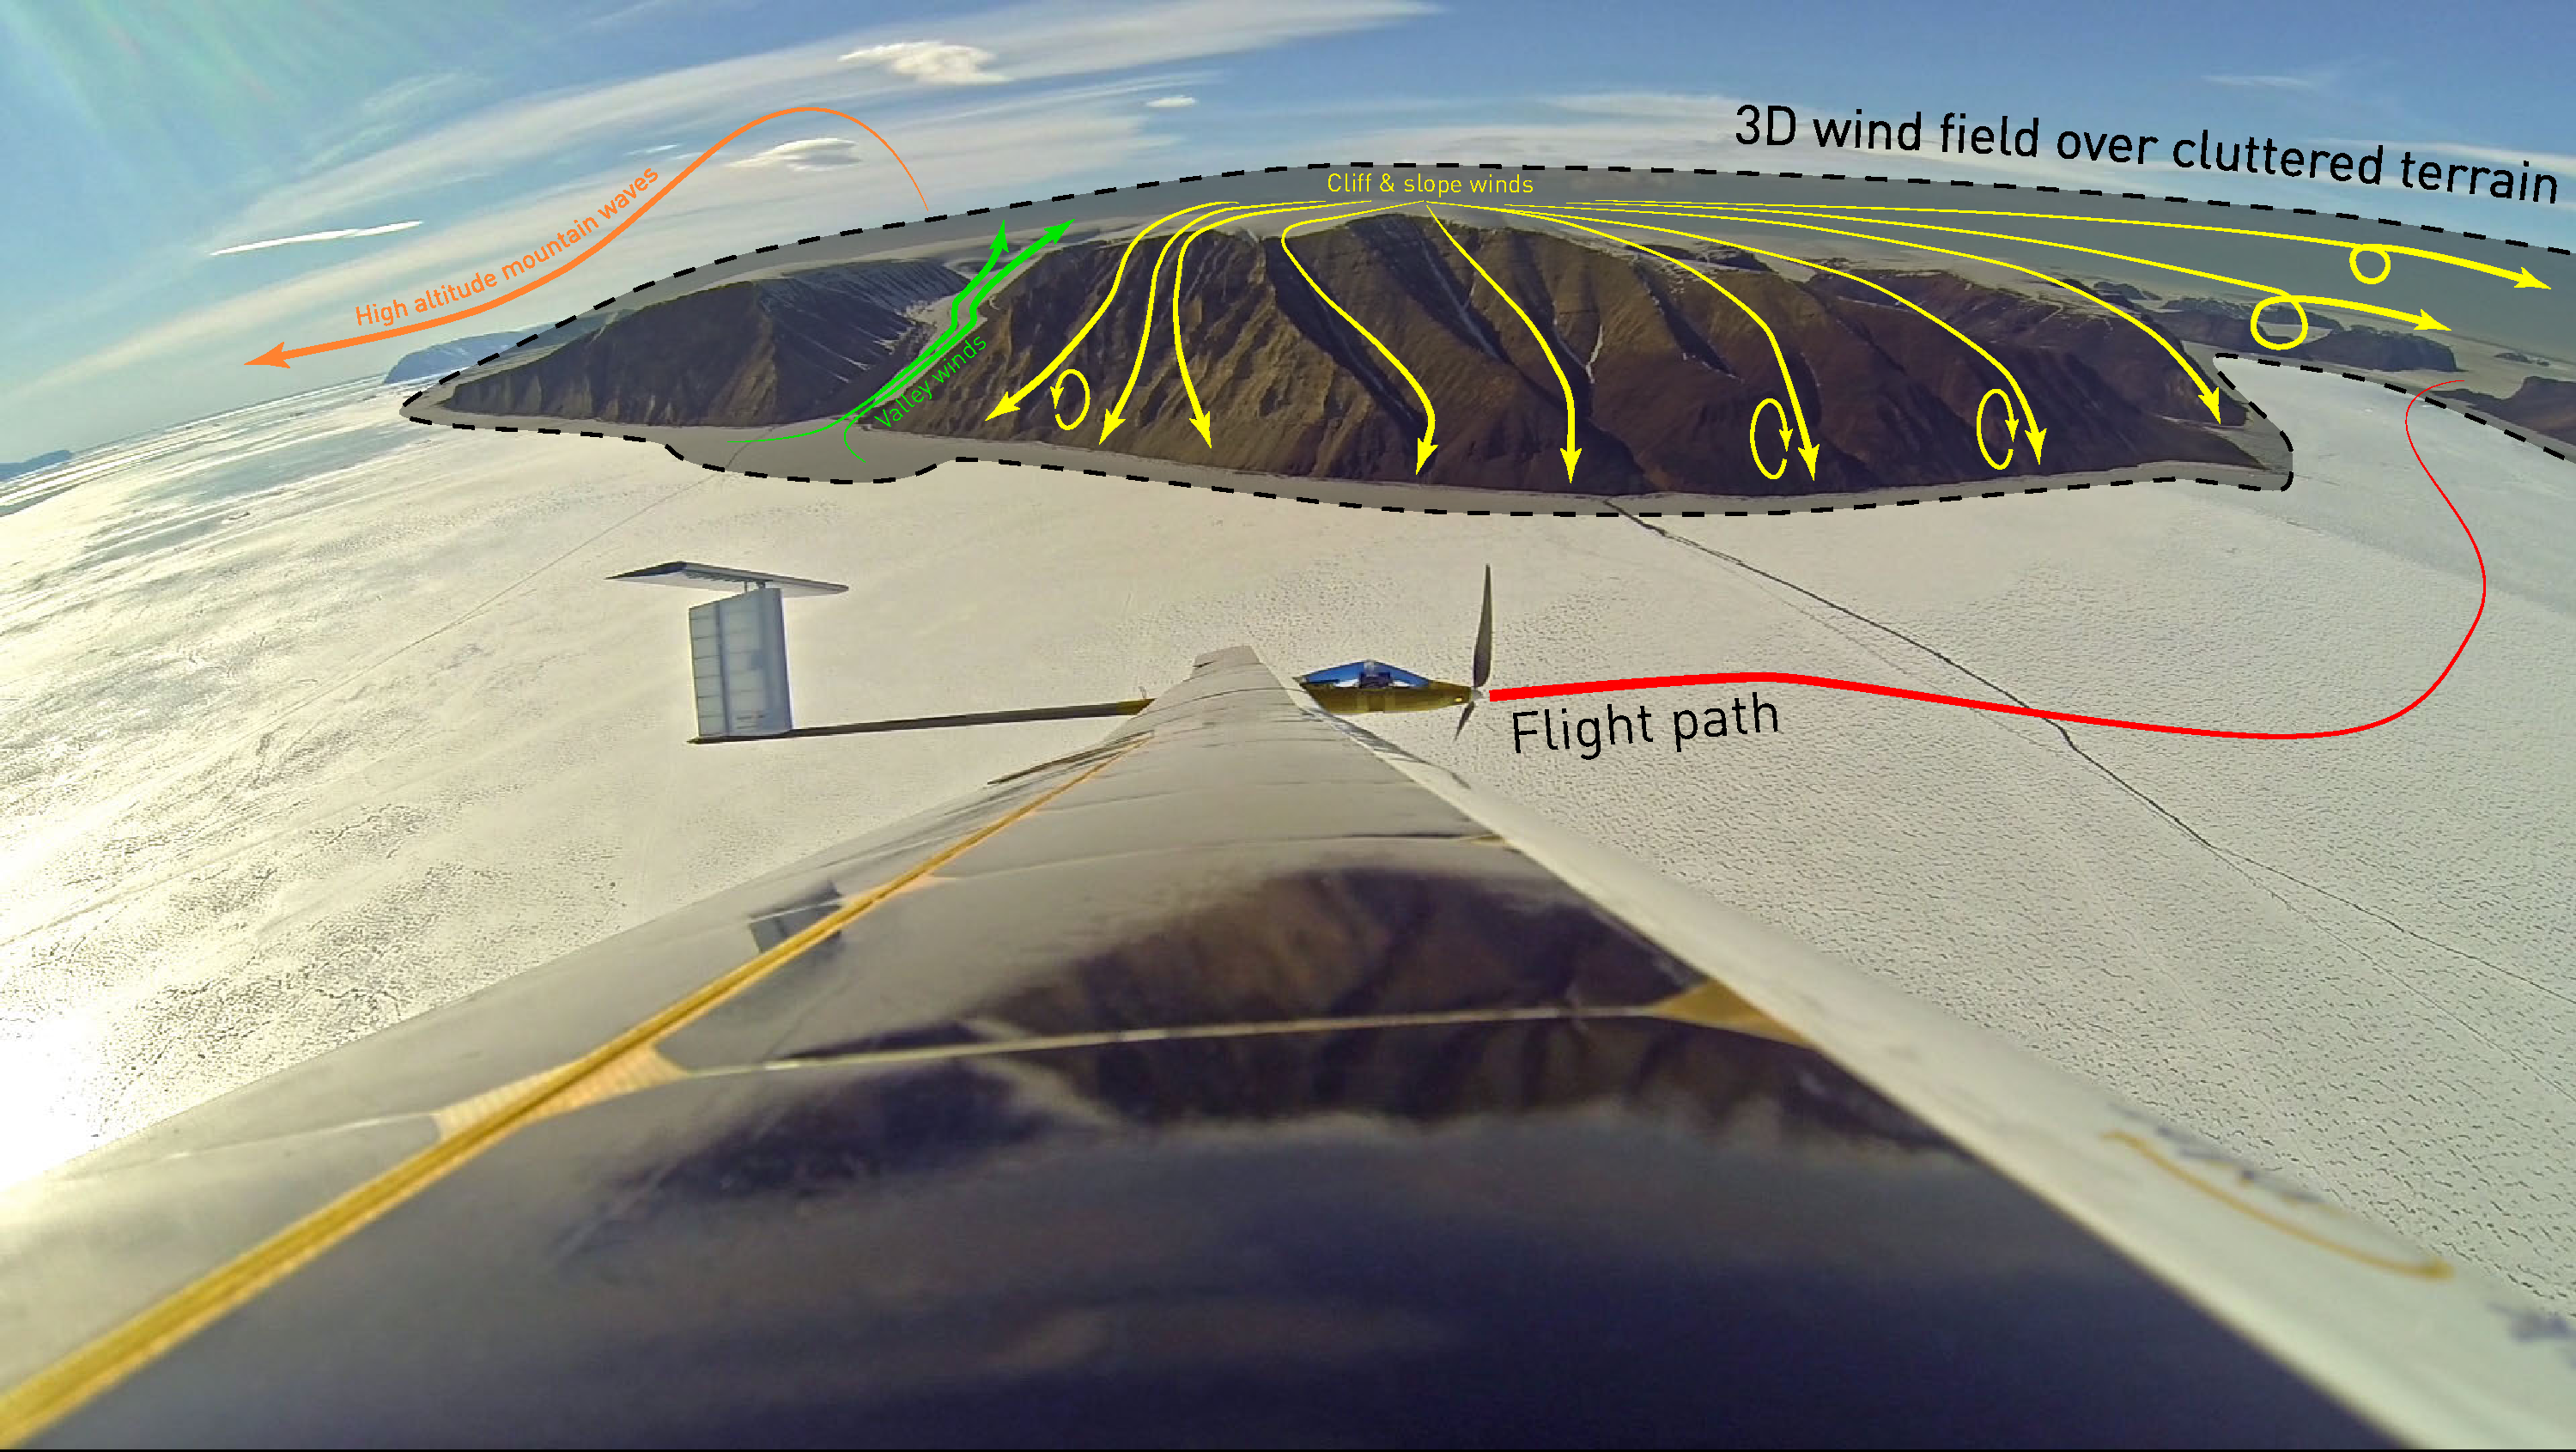
\includegraphics[width=\columnwidth]{images/Introduction/Collage2}
\caption{
Cluttered terrain and strong winds, as e.g. observed in the pictured operation of \emph{AtlantikSolar}~\protect\cite{Oettershagen2018Metpass,Oettershagen_JFR2017} above the Arctic, pose a significant risk to a \ac{UAV}. This paper therefore presents a downscaling method to predict the local 3D wind field in real time such that path planners can calculate optimal trajectories throughout complex terrain and wind.
}
\label{fig:PL_Intro_Collage}
\end{figure}

Safe operations in such complex environments require three technologies that do not exist together on today's small-scale UAVs: First, a \ac{SLAM} system to create a map of the environment, second, a method to predict the local 3D wind field around the \ac{UAV}, and third, a path planner to calculate an optimal collision-free path through the terrain and 3Dnwind field. The focus of this paper is on wind field prediction. Such a system needs to run in real time to react to new terrain information. In addition, to guarantee flight safety at all times, including conditions with a degraded communication link, the system needs to run onboard and be independent from local infrastructure.

%%%%%%%%%%%%%%%%%%%%%%%%%%%%%%%%%%%%%%%%%%%%%%%%%%%%%%%%%%%%%%%%%
\subsection{Contributions}
\label{sec:PL_Intro_Contributions}
%%%%%%%%%%%%%%%%%%%%%%%%%%%%%%%%%%%%%%%%%%%%%%%%%%%%%%%%%%%%%%%%%

This paper presents the literature's first \emph{real-time}\footnote{We define real time as follows: Assume the UAV is flying and constantly mapping previously unknown terrain at a distance $d$ in front of it. Both the wind prediction and path planning then need to be fast enough to allow the UAV to react to potential dangers (obstacles, winds) at distance $d$. For example, if $d=\unit[300]{m}$ and the flight speed is \unitfrac[10]{m}{s}, then calculation times $t\ll\unit[30]{s}$ are considered real time. Real time capability is easier to reach when flying far away from terrain at high altitude where $d$ is also larger.} 3D wind field prediction method that runs directly onboard the limited computational resources of the \ac{UAV}'s onboard computer. The selected downscaling method receives low-resolution \ac{NWP} data as an input via low-bandwidth data links (e.g. satellite communication) and then leverages potential flow theory to generate a high-resolution 3D wind field close to the \ac{UAV}. The method is assessed in simulations and with LIDAR wind profiles from Swiss alpine regions.

Given that this paper is the first in the literature to implement \emph{real-time} 3D wind field predictions \emph{from onboard a \ac{UAV}}, we consider the paper initial work on the path towards full onboard weather-awareness of UAVs. It is not expected that the simple downscaling method captures all the different flow patterns over complex terrain. From a scientific viewpoint, the paper instead seeks to assess how accurately even this simple method can predict the wind field when running onboard a \ac{UAV} in real time and whether this is already enough to allow significant trajectory planning improvements.

%%%%%%%%%%%%%%%%%%%%%%%%%%%%%%%%%%%%%%%%%%%%%%%%%%%%%%%%%%%%%%%%%
\subsection{Organization}
\label{sec:PL_Intro_Contributions}
%%%%%%%%%%%%%%%%%%%%%%%%%%%%%%%%%%%%%%%%%%%%%%%%%%%%%%%%%%%%%%%%%

The remainder of this paper is organized as follows. \Cref{sec:PL_WindPred_StateOfTheArt} presents the current state of the art. \Cref{sec:PL_WindPred_MethodSelection} defines the method requirements and presents the design of the selected method. \Cref{sec:PL_WindPred_Results} presents both synthetic and experimental results. \Cref{sec:PL_WindPred_Conclusion} concludes the paper.

%%%%%%%%%%%%%%%%%%%%%%%%%%%%%%%%%%%%%%%%%%%%%%%%%%%%%%%%%%%%%%%%%
\section{State of the Art}
\label{sec:PL_WindPred_StateOfTheArt}
%%%%%%%%%%%%%%%%%%%%%%%%%%%%%%%%%%%%%%%%%%%%%%%%%%%%%%%%%%%%%%%%%

UAV-based \emph{predictions} of wind fields have not been discussed in the current literature yet. Instead, only \emph{in-situ measurement} methods are described: Filtering approaches that fuse the information of an \ac{IMU}, \ac{GPS} and airspeed sensor are mostly used~\cite{Petrich2011WindEstimation,Langelaan2011WindEstimation}. Approaches that estimate the wind vector without an airspeed sensor also exist~\cite{palanthandalam2008WindEstimationWithoutAirspeedSensor}. In addition, formations of UAVs have been used to cooperatively measure wind fields~\cite{Larrabee2014WindEstimationCooperative}. To find suitable methods for the \emph{online prediction} of 3D wind fields from UAVs, \emph{downscaling} methods that historically come from the fields of meteorology and flow simulation are investigated. In general, these downscaling methods are of three different types:

\begin{itemize}
\item \emph{Statistical methods} use previously measured wind data in a certain region and thereof derive wind expectations for the same region using statistical methods. Given that we aim to predict the wind over unvisited terrain, these methods are not suitable for our application.
\item \emph{Prognostic models} calculate the approximate solution of differential equations describing the \ac{ABL}. They can reproduce small-scale weather effects, but are computationally expensive. ARPS, the Advanced Regional Prediction System~\cite{Xue2000,Xue2001}, has been applied to complex terrain \cite{Mott2010,Mott2010b,Hug2005,Raderschall2008} and is freely available\footnote{\url{http://www.caps.ou.edu/ARPS/arpsdown.html}}. GRAMM, the Graz Mesoscale Model~\cite{GRAMM}, considers mass, momentum, potential temperature and humidity conservation and is often used together with the dispersion model GRAL (Graz Lagrangian Model), e.g. in \cite{Oettl2015}. It is free\footnote{\url{http://lampx.tugraz.at/~gral/index.php/download}} and provides a GUI.
\item \emph{Diagnostic methods} do not have a proper physical background but return a physically consistent wind field with respect to mass or momentum conservation. They are less computationally demanding than prognostic models but cannot predict local effects such as slope winds \cite{Ratto1994} or the time-dependency of the flow. MATHEW~\cite{Sherman1978a,Sherman1978b} is a diagnostic mass consistent model which adds a potential field to an initial wind field to make it divergence free. The source code of a modified model is available~\cite{Walt2016}. CALMET~\cite{CALMET} additionally models kinematic terrain effects, slope flows and blocking effects and can incorporate observational data at the cost of increased computational cost. The usage of CALMET coupled to NWP data showed a significant improvement with respect to NWP outputs \cite{Truhetz2007,Morales2012}. Software licences are available for free\footnote{\url{http://www.src.com/calpuff/calpuff_eula.htm}}. WindNinja~\cite{Forthofer2014} provides two different models: A mass-conserving model which resembles MATHEW, and a mass- and momentum-conserving model that uses commercial \ac{CFD} software. Near surface winds are improved especially for high-wind events~\cite{Wagenbrenner2016}. The software with GUI is available for free\footnote{\url{https://www.firelab.org/document/windninja-software}}.
\end{itemize}

%%%%%%%%%%%%%%%%%%%%%%%%%%%%%%%%%%%%%%%%%%%%%%%%%%%%%%%%%%%%%%%%%
\section{Method Design}
\label{sec:PL_WindPred_MethodSelection}
%%%%%%%%%%%%%%%%%%%%%%%%%%%%%%%%%%%%%%%%%%%%%%%%%%%%%%%%%%%%%%%%%

%%%%%%%%%%%%%%%%%%%%%%%%%%%%%%%%%%%%%%%%%%%%%%%%%%%%%%%%%%%%%%%%%
%\subsection{Method Selection}
%\label{sec:PL_WindPred_MethodSelection}
%%%%%%%%%%%%%%%%%%%%%%%%%%%%%%%%%%%%%%%%%%%%%%%%%%%%%%%%%%%%%%%%%

\subsection{Requirements}

The following specific requirements are derived for the UAV-based wind prediction framework: It shall

\begin{itemize}
\item be usable on UAVs operating remotely or in cluttered terrain where the communication to the ground station is limited or even completely lost. An onboard-implementation is therefore required.
\item provide results in near real-time, i.e. shall calculate a sufficiently accurate 3D wind field for an area of $\unit[1]{km^3}$ (with the \ac{UAV} at its center) and \unit[25]{m} grid resolution in less than \unit[30]{s} calculation time on the UAV's onboard computer\footnote{Such as an INTEL UP Board, \url{http://www.up-board.org/up/}}. We assume this corresponds to \unit[10]{s} on a standard laptop computer.
\item have a robust and fully automated execution that does not require any human intervention.
\item be modular and easily modifiable.
\end{itemize}

\subsection{Selection}

Five different models were traded off against the requirements presented above. First, both ARPS and GRAMM/GRAL were discarded because they violate the computation time constraint, i.e. usually require far more time to guarantee that a numerically stable solution is reached. The mass- and momentum-conserving version of WindNinja is discarded due to computation time disadvantages, too. Of the remaining models, CALMET is considered slower and has a less modular code base. The two remaining models are MATHEW and the mass-conserving WindNinja, which essentially solve the same mathematical problem. Finally, MATHEW is selected because it has a slim and modular source code and can, as shown by Walt~\cite{Walt2016}, solve similar meteorological downscaling problems within the calculation time requirements. In addition, it solves the internal finite element problem using FEniCS, an open-source library that already provides many different solvers and preconditioners, has both Python and C++ bindings, and supports various grid types.

%%%%%%%%%%%%%%%%%%%%%%%%%%%%%%%%%%%%%%%%%%%%%%%%%%%%%%%%%%%%%%%%%
\subsection{Fundamentals}
\label{sec:PL_WindPred_Fundamentals}
%%%%%%%%%%%%%%%%%%%%%%%%%%%%%%%%%%%%%%%%%%%%%%%%%%%%%%%%%%%%%%%%%

%\subsection{Mathematical derivation}
%\label{sec:PL_WindPred_mathematical_derivation}

MATHEW calculates the divergence-free wind field $\vec{u}$ from an initial wind field $\vec{u}^\text{I}$ (retrieved from a NWP system), a \ac{DEM} and the stability matrix $\matr{S}$. The problem domain $\Omega$ is an open set in 3-dimensional space and its boundaries are the Dirichlet boundary $\Gamma_\text{D}$, which covers the open-flow boundary, and the Neumann boundary $\Gamma_\text{N}$ defining the terrain (\cref{fig:PL_WindPred_Fund_Grid2D}). 
	\begin{figure}[b]
	\centering
	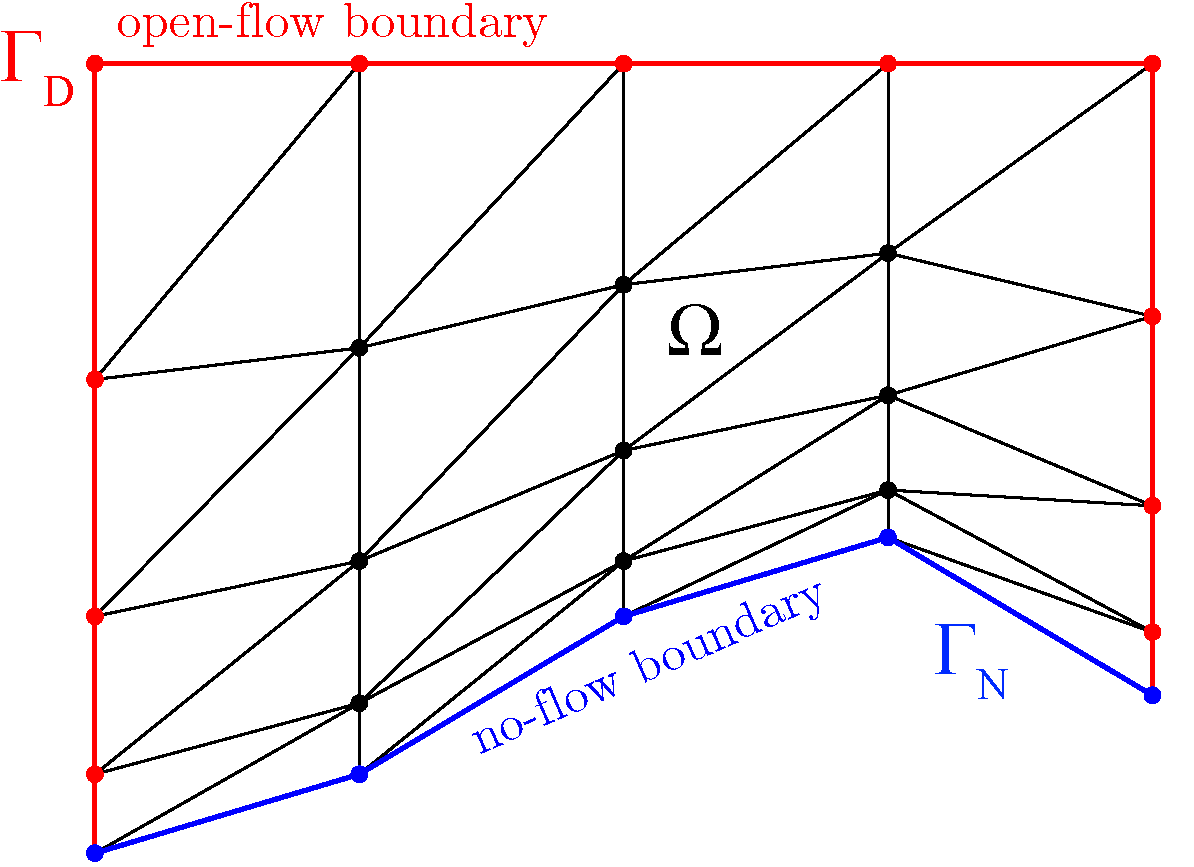
\includegraphics[width=0.8\columnwidth]{images/WindPred/Fundamentals/grid.pdf}
	\caption[2D grid]{Computational domain and boundaries of MATHEW on a 2D grid: The red lines and dots represent the open-flow boundary whereas blue is used for the terrain. The black dots are the grid points within the domain $\Omega$ and the black lines illustrate the cells.}
	\label{fig:PL_WindPred_Fund_Grid2D}
	\end{figure}
The central \emph{hard} constraint enforced by MATHEW is that the resulting $\vec{u}$ needs to be divergence free over the domain $\Omega$, i.e.
	\begin{equation}
	\nabla \cdot \vec{u} = 0\; .
	\label{eqn:PL_WindPred_wind_div_free}
	\end{equation}
This essentially means that the flow is incompressible. The main \emph{soft} constraint is that the adjustments between the initial wind field $\vec{u}^\text{I}$ and the final wind field $\vec{u}$ shall be minimal. This expresses the assumption that the initial wind field observation $\vec{u}^\text{I}$ contains valuable information collected through sensing or a prior model --- and is thus \emph{to some degree} correct (see \cref{sec:PL_WindPred_PrelResults_Synthetic} for a violation of that assumption). Mathematically, MATHEW reduces the accumulated error between $\vec{u}$ and $\vec{u}^\text{I}$ over the domain in a least-squares sense by minimizing the functional
	\begin{equation}
	\pazocal{L}(\vec{u}; \lambda) = \int\limits_{\Omega} \left( \frac{1}{2} \matr{S} \left( \vec{u} - \vec{u}^\text{I} \right) \cdot \left( \vec{u} - \vec{u}^\text{I} \right) + \lambda \nabla \cdot \vec{u} \right)dV \; , 
	\label{eqn:PL_WindPred_functional}
	\end{equation}
with velocity potential $\lambda$ and the atmospheric stability matrix
	\begin{equation}
	\matr{S} = \begin{pmatrix}
	\alpha_\text{h}^2 & 0 & 0 \\ 0 & \alpha_\text{h}^2 & 0 \\ 0 & 0 & \alpha_\text{v}^2
	\end{pmatrix} \; .
	\label{eqn:PL_WindPred_stab_mat}
	\end{equation}
Here, $\alpha_\text{h}$ and $\alpha_\text{v}$ are weights for the horizontal and vertical component. In contrast to the work by Sherman~\cite{Sherman1978a}, they are herein defined as $\alpha_i^2=1/\sigma_i^2$, where $\sigma_i$ are the observation errors or deviations of the observed and desired wind field. The weights $\alpha_\text{h}$ and $\alpha_\text{v}$ are used to define the stability parameter $\alpha$ as 
	\begin{equation}
	\alpha = \frac{\alpha_\text{h}^2}{\alpha_\text{v}^2} = \left( \frac{w}{u} \right)^2 \; ,
	\end{equation}
where $u$ and $w$ are the magnitudes of the expected horizontal and vertical wind speeds, respectively. Inserting $\alpha$ into the definition of the stability matrix, its inverse becomes
	\begin{equation}
	\matr{S}^{-1} = c\cdot\begin{pmatrix}
	1 & 0 & 0 \\ 0 & 1 & 0 \\ 0 & 0 & \alpha
	\end{pmatrix} \; .
	\end{equation}
Note that the constant factor $c$ is neglected ($c=1$) in \cite{Walt2016,Mueller_MT_WindPrediction} because it, first, does not have an effect on the final wind field $\vec{u}$ as during the solution of \cref{eqn:PL_WindPred_weak_form} $\lambda$ would automatically be scaled by 1/c, and second, it cannot be used to adjust the atmospheric stability. This is however possible using the stability parameter $\alpha$. Sherman~\cite{Sherman1978a} assesses multiple test cases and determines a typical value of $\alpha \approx 10^{-4}$. A larger $\alpha$ implies that the wind field is mainly corrected in vertical direction, a smaller one that the correction is principally applied to the horizontal direction.

To minimize \cref{eqn:PL_WindPred_functional}, we apply the Euler-Lagrange equations for vector functions 
\begin{equation}
\frac{\partial\pazocal{L}}{\partial f_i}-\frac{d}{dx} \Big( \frac{\partial\pazocal{L}}{\partial f_i^\prime}\Big) = 0 \; .
\end{equation}
The problem definition now has the form 
\begin{equation}
	\vec{u} = \vec{u}^\text{I} + \matr{S}^{-1} \nabla \lambda \; .
	\label{eqn:PL_WindPred_wind_pred}
\end{equation}
Note that while the added potential flow field $S^{-1}\nabla\lambda$ in \cref{eqn:PL_WindPred_wind_pred} is vorticity-free, the final wind field $\vec{u}$ can still contain vorticity (for example recirculation behind a ridge) if it is already present in $\vec{u}^\text{I}$. Two boundary conditions are now applied: The no-flow through terrain assumption, which translates to $\vec{u}\cdot\vec{n}=0$ where $\vec{n}$ is the normal vector at the terrain, and the assumption of no adjustment of the tangential velocities at the open-flow boundaries, which translates to $\lambda=0$. The resulting system of equations is
	\begin{equation}
	\begin{aligned}
	\vec{u} &= \vec{u}^\text{I} + \matr{S}^{-1} \nabla \lambda && \text{in } \Omega \\
	\nabla \cdot \vec{u} &= 0 && \text{in } \Omega \\
	\lambda &= 0 && \text{on } \Gamma_\text{D} \\
	\vec{u} \cdot \vec{n} &= 0 && \text{on } \Gamma_\text{N} \; .
	\label{eqn:PL_WindPred_problem_orig}
	\end{aligned}
	\end{equation}
These equations can be expressed as a \ac{PDE} for the velocity potential $\lambda$ by taking the scalar product with the gradient operator on both sides of \cref{eqn:PL_WindPred_problem_orig}:
	\begin{equation}
	\begin{aligned}
	-\nabla \cdot \left(\matr{S}^{-1} \nabla \lambda\right) & = \nabla \cdot \vec{u}^\text{I} && \text{in } \Omega \\
	\lambda &= 0 && \text{on } \Gamma_\text{D} \\
	\left(-\matr{S}^{-1} \nabla \lambda\right) \cdot \vec{n} &= \vec{u}^\text{I} \cdot \vec{n} && \text{on } \Gamma_\text{N} \; .
	\label{eqn:PL_WindPred_problem_pdf}
	\end{aligned}
	\end{equation}
\Cref{eqn:PL_WindPred_problem_pdf} is an elliptic \ac{PDE}. For the transformation into a \ac{FEM} problem, the first line in \cref{eqn:PL_WindPred_problem_pdf} needs to be post-multiplied with a test function $\pazocal{F}$ satisfying its boundary condition ($\pazocal{F} = 0$ on $\Gamma_\text{D}$) and integrated over the problem domain $\Omega$:
	\begin{align}
	- \int\limits_{\Omega} \nabla \cdot \left(\matr{S}^{-1} \nabla \lambda\right) \pazocal{F} \, dV = \int\limits_{\Omega} \left(\nabla \cdot \vec{u}^\text{I} \right) \pazocal{F} \, dV \; .
	\label{eqn:PL_WindPred_pde_trial}
	\end{align}
Using Green's Theorem on \cref{eqn:PL_WindPred_pde_trial} and rearranging the terms yields the so called weak formulation of the problem
\begin{equation}
	\underbrace{\int\limits_{\Omega} \left( \matr{S}^{-1} \nabla \lambda \right) \! \cdot \! \nabla \pazocal{F} \, dV}_{a(\lambda,\pazocal{F})} = \underbrace{\int\limits_{\Omega} \left( \nabla \! \cdot \! \vec{u}^\text{I} \right) \pazocal{F} \, dV - \int\limits_{\Gamma_\text{N}} \left( \vec{u}^\text{I} \! \cdot \! \vec{n} \right) \pazocal{F} \, dS}_{l(\pazocal{F})}
	\label{eqn:PL_WindPred_weak_form}
	\end{equation}
Here, $a(\lambda,\pazocal{F})$ is the bilinear form and $l(\pazocal{F})$ is the linear form. The procedure is to now solve for the velocity potential $\lambda$ using the Ritz-Galerkin discretization (for details see Walt~\cite{Walt2016}), and to finally re-insert $\lambda$ into \cref{eqn:PL_WindPred_wind_pred} to retrieve the final 3D wind field $\vec{u}$.

%%%%%%%%%%%%%%%%%%%%%%%%%%%%%%%%%%%%%%%%%%%%%%%%%%%%%%%%%%%%%%%%%
\subsection{Implementation}
\label{sec:PL_WindPred_Implementation}
%%%%%%%%%%%%%%%%%%%%%%%%%%%%%%%%%%%%%%%%%%%%%%%%%%%%%%%%%%%%%%%%%

%\paragraph{Architecture}

\Cref{fig:PL_WindPred_Impl_Architecture} presents the data sources and steps required by our implementation of MATHEW. The framework is implemented in Python with \ac{ROS} support. The input data are the simulation parameters, a \ac{DEM} and coarse \ac{NWP} data (wind profiles around and within the region of interest). The input data is monitored at \unit[0.5]{Hz} and the model is initialized when the inputs have changed. The grid is generated and the initial wind field $\vec{u}^\text{I}$ is calculated by linearly interpolating the coarse \ac{NWP} data to the vertical layer heights of the high-resolution grid. Afterwards bilinear interpolation is used within each vertical layer to calculate the wind components at each grid point. After setting up the weak problem formulation and solving for the velocity potential $\lambda$, the final wind field $\vec{u}$ is then calculated using \cref{eqn:PL_WindPred_wind_pred} and forwarded to a flight planner as described in \cite{Oettershagen2018RealTimePlanning}.

\begin{figure}[htb]
\centering
\tikzstyle{base} = [draw, text width=5em, minimum height=3.5em]
\tikzstyle{process} = [base, rectangle, text centered, text width=10em, minimum height=3em, fill=blue!15]
\tikzstyle{extprocess} = [base, rectangle, text centered, text width=10em, minimum height=3em, fill=green!15]
\tikzstyle{inout} = [base, trapezium, trapezium left angle=70, trapezium right angle=-70, text badly centered, trapezium stretches=true, fill=orange!15]
\tikzstyle{line} = [draw, -latex']

\begin{tikzpicture}[node distance=1.2cm, scale=0.75, every node/.style={transform shape}]
\node [inout] (nwp) {NWP \\ data};
\node [inout, left of=nwp, node distance=2.2cm] (dem) {DEM \\ data};
\node [inout, right of=nwp, node distance=2.2cm] (simparam) {simulation parameters};

\coordinate [below of=nwp, node distance=0.8cm] (inputs);

\node [extprocess, below of=inputs, node distance=0.8cm] (updated) {updated?};
\coordinate [right of=updated, node distance=2.5cm] (updatedDecision);
\coordinate [below of=updatedDecision,node distance=1.2cm] (updatedDecisionNo1);
\coordinate [below of=updated,node distance=1.2cm] (updatedDecisionNo2);

\node [process, right of=updatedDecision, node distance=3.0cm] (init) {initialize model with DEM, NWP and simulation parameters};
\node [process, below of=init, node distance=4.2em] (grid) {create grid and interpolate NWP data to its nodes};
\node [process, below of=grid, node distance=3.9em] (fem_setup) {set up weak formulation of FEM problem \eqref{eqn:PL_WindPred_weak_form}};
\node [process, below of=fem_setup, node distance=3.8em] (vel_pot) {solve for velocity potential $\lambda$};
\node [process, below of=vel_pot, node distance=3.8em] (pred) {add potential field to initial wind field \eqref{eqn:PL_WindPred_wind_pred}};
\node [inout, left of=pred, node distance=5.5cm] (windfield) {adjusted wind field};
\node [extprocess, below of=windfield,node distance=1.4cm] (planner) {flight planner};

\path [line] (dem) |- (inputs) -- (updated);
\path [line] (nwp) -- (updated);
\path [line] (simparam) |- (inputs) -- (updated);
\path [draw] (updated) -- (updatedDecision);
\path [line] (updatedDecision) |- (updatedDecisionNo2) -- (updated);
\path (updatedDecision) edge node[right]{No} (updatedDecisionNo1);
\path (updatedDecisionNo1) edge node [above,color=gray]{0.5 Hz} (updatedDecisionNo2);

\path (updatedDecision) edge[-latex'] node[above]{Yes} (init);
\path [line] (init) -- (grid);
\path [line] (grid) -- (fem_setup);
\path [line] (fem_setup) -- (vel_pot);
\path [line] (vel_pot) -- (pred);
\path [line] (pred) -- (windfield);
\path [line] (windfield) -- (planner);
\path [line] (windfield) -- (updated);

%Legend %0.35
\node (legend_data) at ( 6.9,-8.2) [text width=2em, minimum height=1em, fill=orange!15,label=left:Data] {};
\node (legend_process) [text width=2em, minimum height=1em, fill=blue!15,below of=legend_data, node distance=0.35cm, label=left:Wind model calculation] {};
\node (legend_extprocess) [text width=2em, minimum height=1em, fill=green!15,below of=legend_process, node distance=0.35cm, label=left:External process] {};

\end{tikzpicture}

%\path [line] (updatedDecisionNo2) -- (updated);
%\path (updatedDecision) | (updated);
%\path [line] (updatedDecision) (init);
%edge["Yes"']
%\path [line] (updatedDecision) -- (init);
\caption[Architecture and interfaces]{Wind downscaling architecture: Input data changes trigger the wind field downscaling calculation, which then publishes its outputs to \ac{ROS} and the flight planner.}
\label{fig:PL_WindPred_Impl_Architecture}
\end{figure}

The decision to implement the architecture of \cref{fig:PL_WindPred_Impl_Architecture} onboard a \ac{UAV} instead of a ground-based computer is motivated by the requirement to have wind field forecasts available at all times, i.e. even when flying remotely with reduced communication bandwidth to the ground station. The transmitted data volume therefore needs to be minimal. However, even the $\unit[1]{km^3}$ high-resolution wind field defined in \cref{sec:PL_WindPred_MethodSelection} contains 1681 horizontal grid points with multiple vertical layers. Calculating this wind field on a ground-based computer and transmitting the results via low-speed telemetry links (for example degraded line-of-sight telemetry or satellite communication) is not possible in real-time. Therefore, an onboard implementation is chosen. The NWP data is provided by the European \ac{COSMO} model~\cite{COSMOMeteoSwiss} at \unit[1--7]{km} horizontal resolution and up to 80 vertical layers. A ground-based client computer only extracts the \ac{NWP} data at the specific time and region of interest. Assuming COSMO-1 \ac{NWP} data, the $\unit[1]{km^3}$ region of interest then consists of only 9 horizontal grid points with different vertical levels that need to be transmitted. Even low-bandwidth links such as the satellite communication link on \emph{AtlantikSolar}~\cite{Oettershagen_JFR2017} can manage such a bandwidth. The \ac{DEM} is either preloaded or generated directly onboard the \ac{UAV} by a vision-based \ac{SLAM} node~\cite{Hinzmann2016}.

\subsection{Optimization}

The framework's accuracy and computation time depend on three critical parameters: The vertical grid point spacing, and the preconditioner and solver used by FEniCS. These are optimized by comparing the model to the analytical results for flow around a hemisphere with radius \unit[0.25]{m} (\cref{fig:PL_WindPred_Impl_HemiError}). It is placed at the origin of the domain $[-1, -1, 0] \times [1, 1, 1]$ (in m) with \unitfrac[1]{m}{s} inflow in positive $x$-direction. $N_x=N_y=41$ horizontal grid points are used. The stability parameter is $\alpha=1$. While the horizontal spacing is constant, the vertical spacing is not: The vertical position $z$ of a grid point at vertical index $n$ and position $x,y$ is defined as
\begin{equation}
z(x, y, n) = h(x, y) + \big(t(x, y) - h(x, y) \big) \cdot \gamma(n) \; ,
\end{equation}
where $h(x, y)$ is the terrain height and $t(x, y)$ is the top vertical domain boundary at the $x,y$ position. The discrete function $\gamma(n)$ needs to be strictly monotonically increasing and fulfill $\gamma(0) = 0$ and $\gamma(N_z) = 1$, where $N_z$ is the number of vertical grid points. Equidistant, square-root, linear and squared spacing functions $\gamma(n)$ are tested. The error at a location is defined as the length of the difference vector between the model output and the analytic solution. The weighed total error sums up the product of each local error with the ratio between the height of the respective cell and the average cell height of the entire domain. The median weighted error for all vertical spacings is nearly the same, i.e. about \unitfrac[0.005]{m}{s}. The linear vertical spacing is selected because its maximum weighted error is only \unitfrac[0.14]{m}{s} and its weighted errors show a low standard deviation.

\begin{figure}[bth]
\centering
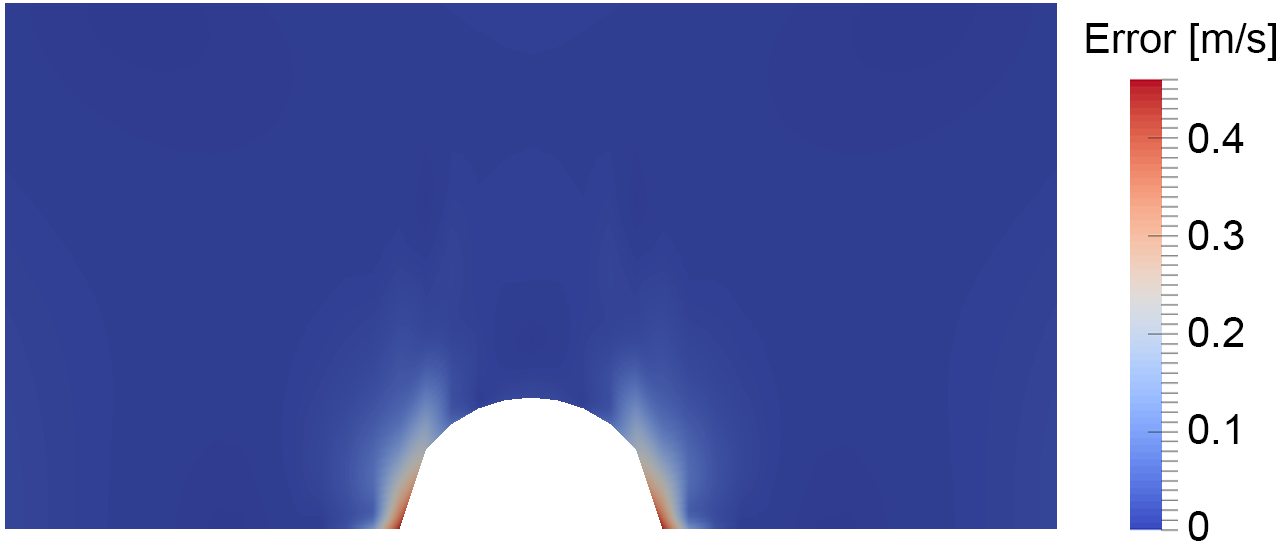
\includegraphics[width=\columnwidth]{images/WindPred/Implementation/error_hemi.png}
\caption[Hemisphere error]{Non-weighted local errors, i.e. the magnitude of the difference between the wind field vectors predicted by the model and the analytical solution, for the hemisphere. The linear vertical spacing, ILU preconditioner and CG solver are used. The largest errors occur in a small region with abrupt terrain change at the bottom of the hemisphere.}
\label{fig:PL_WindPred_Impl_HemiError}
\end{figure}

The elliptic \ac{PDE} of \cref{eqn:PL_WindPred_problem_pdf} was previously solved using a direct solver~\cite{Walt2016}. To fulfill the stringent computation time requirements, different FEniCS preconditioners and iterative solvers were assessed using the aforementioned hemisphere test case. The best combination is found to be the FEniCS Incomplete LU-decomposition (ILU) preconditioner with the Conjugate Gradient (CG) solver. Averaged over 10 runs, this combination reduces the computation time for $\lambda$ from \unit[81.8]{s} for the direct solver to only \unit[6.3]{s}. The $<\unit[10]{s}$ calculation time requirement is thus fulfilled. The additional errors introduced into the wind field have a norm of less than $\unitfrac[10^{-4}]{m}{s}$ and are deemed acceptable given that a time reduction of \unit[92]{\%} is achieved. \Cref{fig:PL_WindPred_Impl_HemiError} shows the overall non-weighted errors of the framework. More detailed information on the implementation and parameter optimization is presented by M{\"u}ller~\cite{Mueller_MT_WindPrediction}.

%%%%%%%%%%%%%%%%%%%%%%%%%%%%%%%%%%%%%%%%%%%%%%%%%%%%%%%%%%%%%%%%%
\section{Results}
\label{sec:PL_WindPred_Results}
%%%%%%%%%%%%%%%%%%%%%%%%%%%%%%%%%%%%%%%%%%%%%%%%%%%%%%%%%%%%%%%%%

%%%%%%%%%%%%%%%%%%%%%%%%%%%%%%%%%%%%%%%%%%%%%%%%%%%%%%%%%%%%%%%%%
\subsection{Synthetic Test Cases}
\label{sec:PL_WindPred_PrelResults_Synthetic}
%%%%%%%%%%%%%%%%%%%%%%%%%%%%%%%%%%%%%%%%%%%%%%%%%%%%%%%%%%%%%%%%%

\subsubsection{Steep and narrow valley}
\label{sec:PL_WindPred_valley}

The steep and narrow valley (\cref{fig:PL_WindPred_valley_testcase}) tests how mass conservation is achieved for different stability parameters. At the center of the valley ($x = 0$, $y = 0$) the width is one fourth of the inflow width. The initial wind field $\vec{u}^\text{I}=[5,0,0]\unitfrac[]{m}{s}$ is constant over the entire domain. While $\vec{u}^\text{I}$ is divergence free over $\Omega$, it violates the terrain boundary conditions. The model output $\vec{u}$ is shown in \cref{fig:PL_WindPred_valley_testcase,fig:PL_wind_fields_valley}. The ratio of the average inflow speed to the average valley wind speed is roughly 1/4, thus mass conservation is fulfilled. The average wind speed in the domain is slightly reduced (\cref{tab:PL_WindPred_wind_valley}). For $\alpha=1.00$, the flow is also able to avoid the orifice represented by the valley by rising in front of the valley and sinking again afterwards. Given the open flow boundary above the valley this behavior is expected. Overall, the test case shows that $\vec{u}$ is made divergence free, terrain following and mass consistent. However, it also shows a major difference to common \ac{CFD} software: \Cref{eqn:PL_WindPred_functional} minimizes the least squares error between $\vec{u}$ and $\vec{u}^\text{I}$ over the whole domain $\Omega$, and this error is smaller if $\vec{u}$ is decreased in the inflow than if it is kept constant at the inflow but significantly increased inside the valley. This process does not respect inflow boundary conditions and significantly changes the mean valley inflow in \cref{tab:PL_WindPred_wind_valley}. Therefore, even if the inflow boundary conditions are known with much higher accuracy than the conditions inside the domain (e.g. from highly accurate NWP data) they are not respected.

\begin{table}[!h]
\caption{Characteristic wind speeds for the valley test and two stability parameters $\alpha$.}
\centering
\begin{tabular}{l r r}
\toprule
Stability parameter & $\alpha = 0.01$ & $\alpha = 1.00$ \\
\midrule
Mean valley inflow [m/s] & 2.32 & 2.75 \\
Maximal wind speed [m/s] & 11.86 & 11.55 \\
Average domain wind [m/s] & 4.48 & 4.62 \\
\bottomrule
\end{tabular}
\label{tab:PL_WindPred_wind_valley}
\end{table}

\begin{figure}[htbp]
\centering
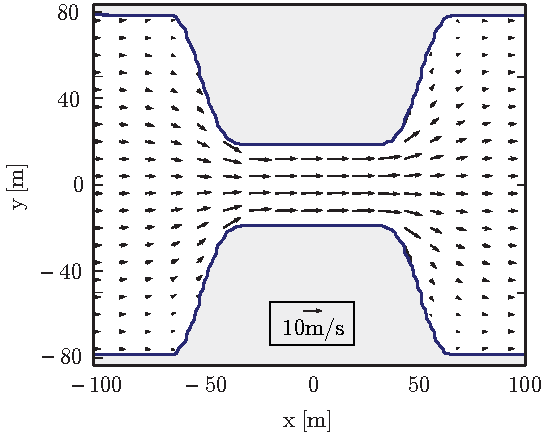
\includegraphics[width=\columnwidth]{images/WindPred/Results/horizontal_flow_valley.pdf}
\caption{Synthetic valley. The terrain height is \unit[0]{m} in the white area and \unit[100]{m} in the grey areas. The adjusted flow (black arrows) is shown at {$z=\unit[40]{m}$} and $\alpha = 1.00$. As expected, the wind speed in the valley is roughly four times as high as at the in and outflow.}
\label{fig:PL_WindPred_valley_testcase}
\end{figure}

\begin{figure}[htbp]
\centering
\subfloat{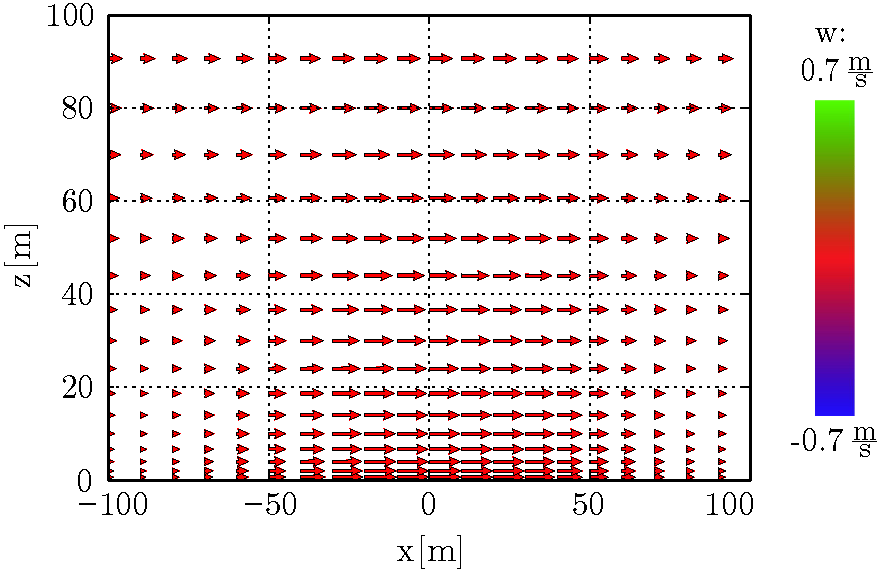
\includegraphics[width=\columnwidth]{images/WindPred/Results/u_pred_valley_alpha0_010000_2.pdf}}
\\
\subfloat{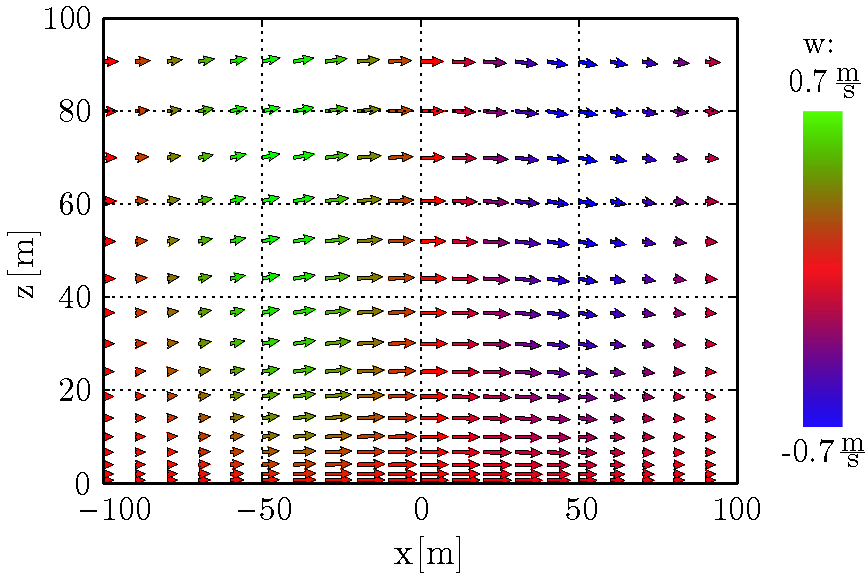
\includegraphics[width=\columnwidth]{images/WindPred/Results/u_pred_valley_alpha1_000000_3.pdf}}
%width=.485\textwidth
\caption{Adjusted wind fields $\vec{u}$ for $\alpha = 0.01$ (top) and $\alpha = 1.00$ (bottom) for the synthetic valley test case in the $x$-$z$ cross section at $y = 0$. The arrow color represents the vertical component $w$. As expected, the wind speed is higher inside the valley. The overall wind magnitude is decreased in both cases. For $\alpha = 1.00$, the flow is also adjusted vertically.}
\label{fig:PL_wind_fields_valley}
\end{figure}

\subsubsection{Ramp}
\label{sec:PL_WindPred_ramp}

The synthetic ramp test case is also initialized with $\vec{u}^\text{I}=[5,0,0]\unitfrac[]{m}{s}$ over the entire domain. The result for a \unit[600]{m} domain height is visualized in \cref{fig:PL_WindPred_ramp_example}. The geometry again represents an orifice for the flow, and the overall wind magnitudes are therefore decreased at the inflow and increased at the outflow. The ratio between inflow and outflow velocities is however lower than in the valley because the geometry narrows less and the top domain boundary is an open flow boundary where some mass is expelled. The vertical flow field and the regions of maximum wind speed close to the top of the ramp --- where soaring flight would be optimal --- are represented well. The comparison with smaller domain heights shows a decrease in quality and emphasizes that MATHEW requires a sufficiently large domain height. For the remaining analysis the domain factor, i.e. the ratio of domain height to the height of the tallest obstacle, is therefore set to 3.5. Overall, the results agree very well with the intuitive solution.

\begin{figure}[htbp]
\centering
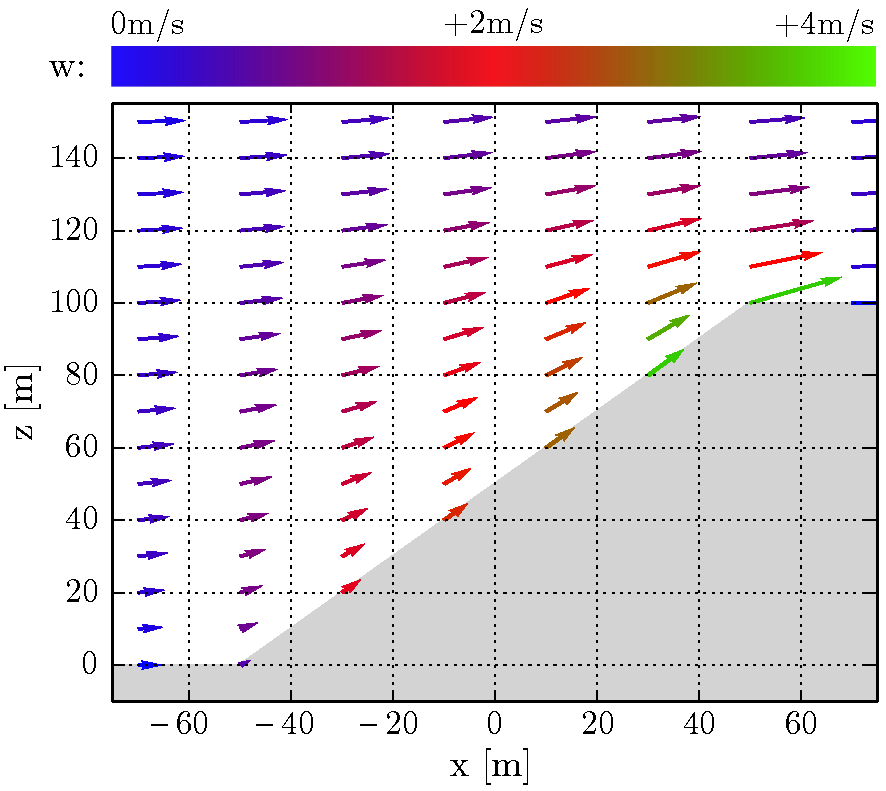
\includegraphics[width=\columnwidth]{images/WindPred/Results/u_pred_ramp_df06_00.pdf}
\caption[Results for the synthetic ramp test case]{Synthetic ramp results: Both the observed flow acceleration and the vertical components $w$ correspond well to an intuitive solution. The arrows scale with the magnitude and the color visualizes $w$. We retrieve {\unitfrac[3.79]{m}{s}} average inflow, {\unitfrac[5.79]{m}{s}} average outflow, {\unitfrac[1.23]{m}{s}} minimal wind, and {\unitfrac[9.69]{m}{s}} maximal wind.}
\label{fig:PL_WindPred_ramp_example}
\end{figure}

%%%%%%%%%%%%%%%%%%%%%%%%%%%%%%%%%%%%%%%%%%%%%%%%%%%%%%%%%%%%%%%%%
\subsection{Experimental Validation}
\label{sec:PL_WindPred_PrelResults_Experimental}
%%%%%%%%%%%%%%%%%%%%%%%%%%%%%%%%%%%%%%%%%%%%%%%%%%%%%%%%%%%%%%%%%

\subsubsection{Measurement and simulation setup}
\label{sec:PL_WindPred_meas_setup}

To compare the model output to actual wind data, an extensive literature review for measured multi-dimensional wind fields in complex terrain and at typical flying altitudes of a \ac{UAV} was performed. Unfortunately, even after multiple weeks of searching no such measurements could be found. Therefore, 1-D LIDAR measurements of wind vectors at multiple altitude levels (\cref{fig:PL_WindPred_vorab_lidar}) are used. The LIDAR data was recorded by the Zurich University of Applied Sciences at three different locations and time periods (\cref{tab:PL_WindPred_campaign_details}). It was filtered and averaged to exclude invalid raw data, missing measurements, or excessive changes within consecutive time steps. More details about the exact instrumentation and measurements can be found in \cite{Kuratle2015} and \cite{Hasler2016} for San Bernardino/Bivio and Vorab, respectively. 

\begin{figure}[htbp]
\centering
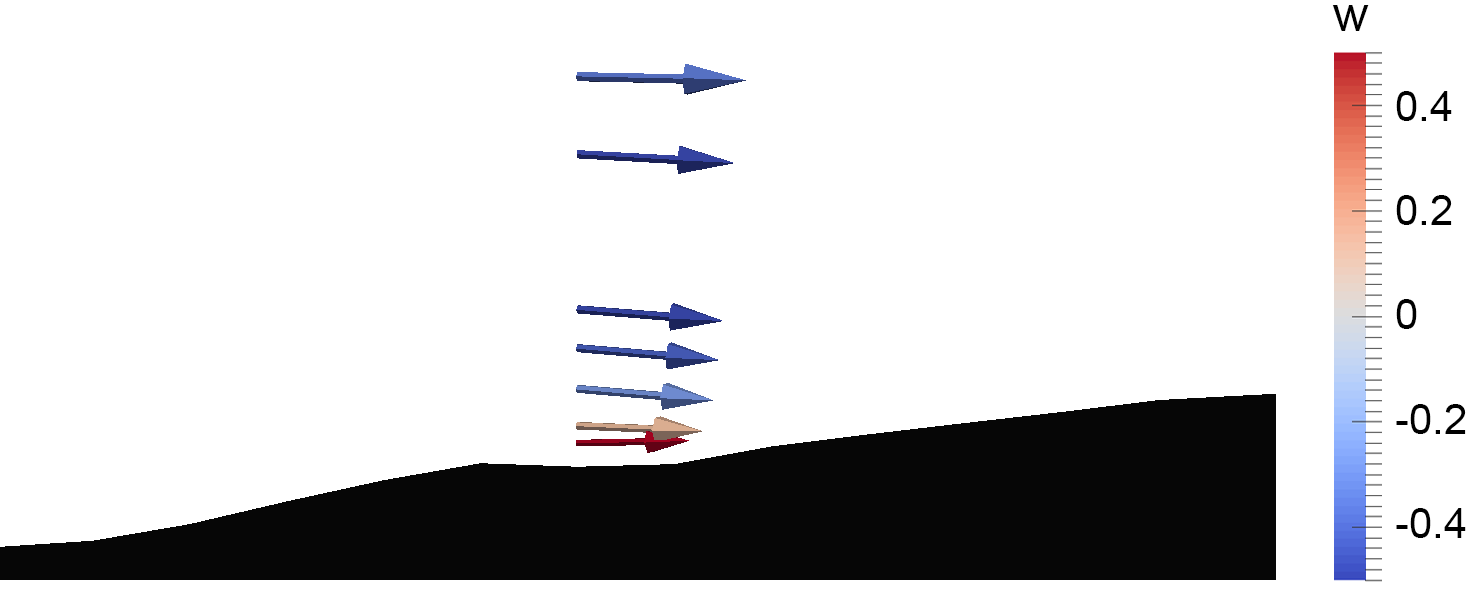
\includegraphics[width=\columnwidth]{images/WindPred/Results/vorab_331_lidar.png}
\caption[LIDAR profile Vorab]{Exemplary LIDAR profile from Vorab with wind vectors at different heights. While we'd expect $w>0$ due to the left-to-right winds and the increasing terrain height in that direction, the LIDAR yields $w<0$ for most altitudes. Such \emph{unintuitive} LIDAR measurements occur regularly. They can be caused by terrain or effects that lie outside the computational domain (e.g. large mountain-waves), which the downscaling model can of course not take into account.}
\label{fig:PL_WindPred_vorab_lidar}
\end{figure}

\begin{table}[htb]
\centering
\caption{LIDAR measurement sites in Switzerland, time periods and amount of valid data (where \emph{d}=days and \emph{p} = LIDAR profiles). The valid data days are less than the time period because data had to be filtered out e.g. due to weather.}

\begin{tabular}{l l l l}
\toprule 
 & San Bern. & Bivio & Vorab\\[0.8ex]
\midrule
Lat.~$^\circ$N & 46.46357 & 46.46251 & 46.87398 \\
Lon.~$^\circ$E & 9.18465 & 9.66864 & 9.18186 \\
Year & 2015 & 2015 & 2016 \\
Period &  Jun.2--Jun.17 & Jun.17--Jul.21 & Mar.22--Apr.4 \\ 
Valid data & 2d/30p & 2d/36p & 6d/70p\\ 
\bottomrule
\end{tabular}

\label{tab:PL_WindPred_campaign_details}
\end{table}

\Cref{fig:PL_WindPred_terrains} visualizes the terrain, the computational domain and the LIDAR, which is always positioned at the center of the computational domain with side length \unit[2.2]{km}. A grid with 20 vertical layers and \unit[50]{m} horizontal resolution is used. Note that for San Bernardino and Bivio only COSMO-2 weather data is available, while the higher-resolution COSMO-1 data can be used for Vorab.

\begin{figure}[htbp]
\centering
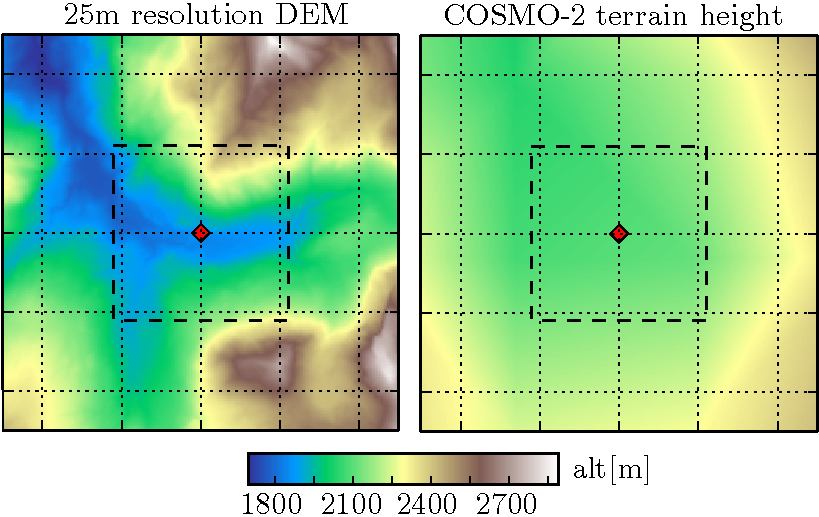
\includegraphics[width=\columnwidth]{images/WindPred/Results/terrain_bivio2.pdf}
\caption[Terrain measurement locations]{Terrain (\unit[5x5]{km}), downscaling domain (\unit[2.2x2.2]{km}, dashed line) and LIDAR location (red diamond) for the Bivio measurement site. North is up. The COSMO-2 terrain is not able to resolve the cluttered terrain. The initial wind field $\vec{u}^\text{I}$ provided by COSMO-2 will thus not be a good approximation of $\vec{u}$. DEM data: \copyright{} 2016 swisstopo (JD100042), free for educational purposes.}
\label{fig:PL_WindPred_terrains}
\end{figure}

\subsubsection{Measured and estimated wind fields}
\label{sec:PL_WindPred_phenomena}

To show how the downscaling model can improve the wind field estimate, but to also show its limitations with respect to modelling small-scale thermally induced wind phenomena, this section exemplarily compares the model output and measured winds for Bivio. As visible in \cref{fig:PL_WindPred_terrains} the LIDAR is located in a steep east-west valley but the corresponding COSMO-2 terrain is basically flat. As a result, on July 8th 9:00 UTC the interpolated COSMO-2 wind field indicates flow coming from south-east (\cref{fig:PL_WindPred_valley_breeze}) and therefore violates the assumption of no flow through the terrain boundaries. The downscaling model is able to rotate $\vec{u}$ in the correct direction such that the winds satisfy the terrain boundary conditions. The measured wind direction agrees well with the downscaled wind field. However, the wind speed is significantly underestimated both by the initial wind field and the adjusted wind field. The overall observed situation is a so called mountain breeze, i.e. a cold air mass that moves from the mountain into the valley during the night and early morning hours. 

\begin{figure}[htbp]
\centering
\subfloat{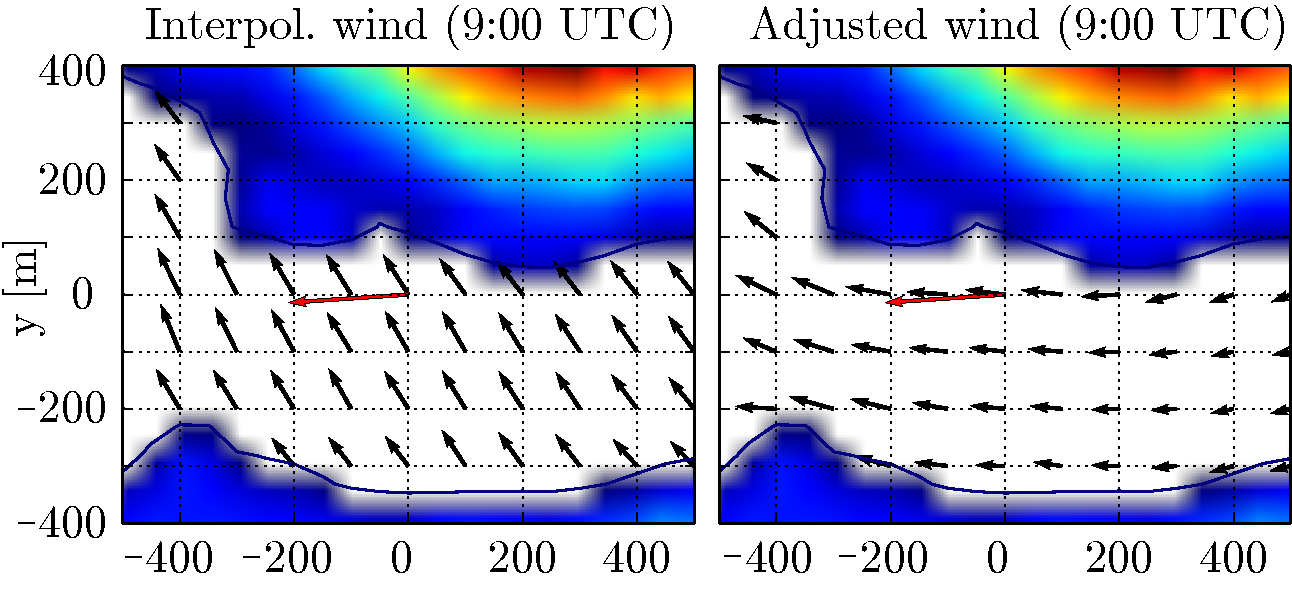
\includegraphics[width=\columnwidth]{images/WindPred/Results/zslice-20150708-09-00_000100-i0162.pdf}}\\[0.7ex]%[-2ex]
\subfloat{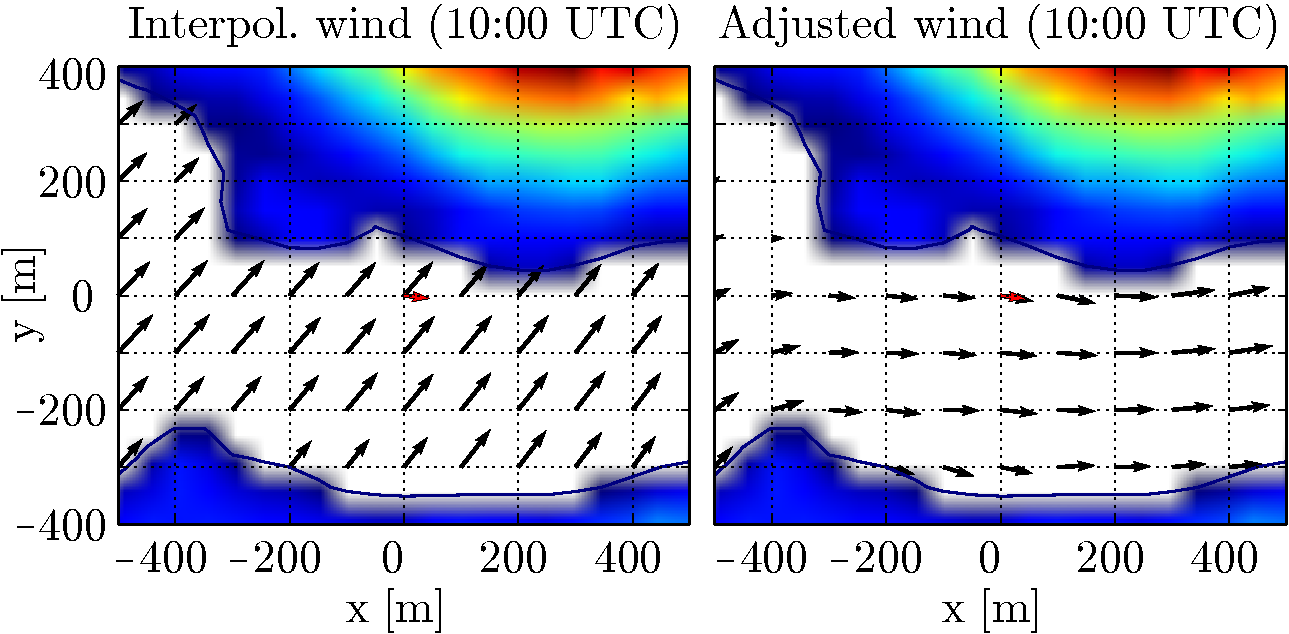
\includegraphics[width=\columnwidth]{images/WindPred/Results/zslice-20150708-10-00_000100-i0170.pdf}}
\caption[Valley breeze Bivio]{Initial and adjusted wind fields $\vec{u}$ (black arrows) at Bivio for 09:00UTC (top) and 10:00UTC (bottom) on July 8th 2015. The wind is shown at \unit[1900]{m} AMSL. The red arrow is the wind measured by the LIDAR.}
\label{fig:PL_WindPred_valley_breeze}
\end{figure}

One hour later, at 10:00 UTC, the wind direction has changed and wind is flowing from the valley to the mountains. This \emph{valley breeze} situation is shown in \cref{fig:PL_WindPred_valley_breeze}. The interpolated wind direction again does not respect the terrain boundaries and also differs significantly from the measured wind direction. The downscaling model is again able to predict the correct wind direction. The wind magnitude is overestimated by both approaches, but the error for the downscaling model is much smaller.

To analyze the reason for the underestimated wind speed at 09:00 UTC, \cref{fig:PL_WindPred_valley_breeze_profile} plots the measured, interpolated and modeled wind profiles. The measured horizontal wind profile shows a distinct maximum \unit[40]{m} above ground. This small-scale phenomenon is called \emph{low-level jet} and is not represented in the interpolated wind profile. Given that the downscaling model has no deeper physical understanding of thermally-induced effects, it also cannot predict this behavior. At 10:00 UTC, the interpolated wind is again too high but the downscaling model can partially correct for this. In both cases, the downscaling model clearly improves the wind direction such that the overall agreement between the modeled and measured wind vectors is improved. 

\begin{figure}[htbp]
\centering
\subfloat{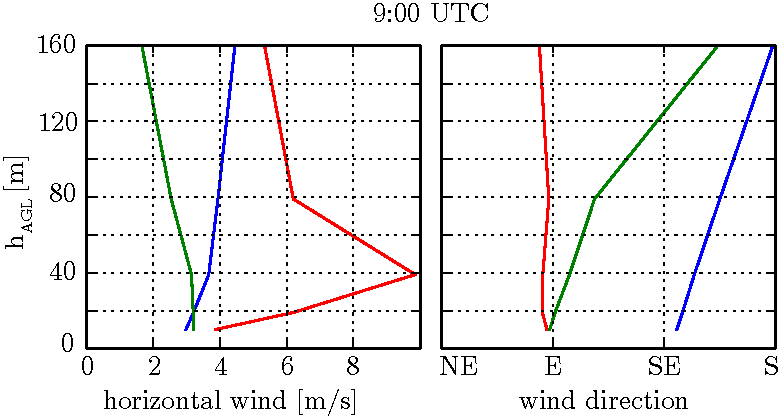
\includegraphics[width=\columnwidth]{images/WindPred/Results/profile_bivio_i0162.pdf}}\\[1.2ex]
\subfloat{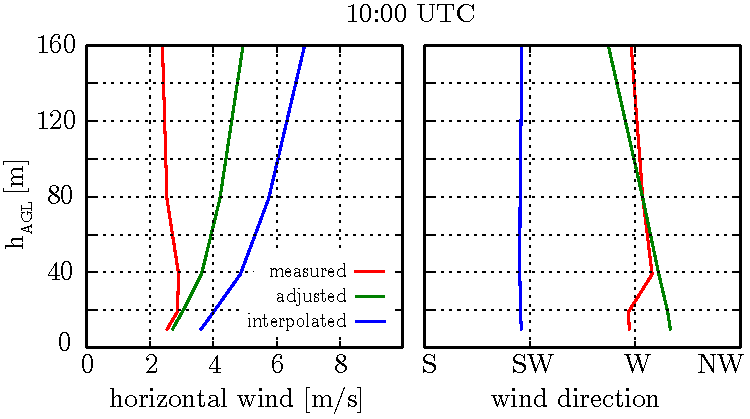
\includegraphics[width=\columnwidth]{images/WindPred/Results/profile_bivio_i0170.pdf}}%\\
%\subfloat{
%\small
%\vspace{10pt}
%\definecolor{darkgreen}{rgb}{0,0.5,0}
%\textcolor{red}{\textbf{---}} measured profile \hspace{10pt} \textcolor{blue}{\textbf{---}} interpolated profile \hspace{10pt} \textcolor{darkgreen}{\textbf{---}} adjusted profile}
\caption{Wind profiles at Bivio on July 8th 2015 at 9:00 UTC (top) and 10:00 UTC (bottom). In the top plot, the LIDAR measures a so-called \emph{low-level jet}. The downscaling model significantly improves the wind direction and tends to improve the wind speed.}
\label{fig:PL_WindPred_valley_breeze_profile}
\end{figure}


\subsubsection{Statistical evaluation}
\label{sec:PL_WindPred_evaluation}

To quantitatively assess the wind field improvement, a comparison of the downscaling model against LIDAR measurements is performed over all test cases. Given that we only want to investigate modeling errors but not errors due to a badly selected stability parameter, we always first run the model for $\alpha = [10^{-6},10^1]$ and select the run with the \emph{optimal} $\alpha$, i.e. the one which yields the minimum \ac{RMSE} between the modeled and measured wind profile. This approach of course has a certain risk of overfitting such that the following results have to be considered best-case results. In the future, the wind field downscaling model will automatically select the best $\alpha$ by assessing the current atmospheric stratification using the temperature profiles in the \ac{NWP} data.

Given that only 1D measurement data exists, all wind fields can only be compared locally at the LIDAR's position. In addition to the downscaled wind field $\vec{u}$, we also compare the initial wind field $\vec{u}^\text{I}$ and a zero-wind field $\vec{u}^0=0$. The LIDAR measurements serve as ground-truth. The comparison metric is the root mean square error. It is calculated for two newly introduced variables: First, the weighted horizontal vector error\footnote{It would make more sense to compare the horizontal wind speed and direction instead of combining them in one variable. But given that the zero wind field $\vec{u}_0$ has no proper wind direction, the above introduced variable seems to be the best solution.} is
	\begin{equation}
	e_\text{hor} = \frac{\sqrt{(u_\text{p} - u_\text{m})^2 + (v_\text{p} - v_\text{m})^2}}{v_\text{air}} \; . 
	\end{equation}
Here, the subscripts $\text{p}$ and $\text{m}$ stand for the predicted and measured components, and $v_\text{air}$ is the nominal airspeed of \unitfrac[9]{m}{s} for \emph{AtlantikSolar}. The variable $e_\text{hor}$ therefore normalizes the horizontal wind estimate error with the aircraft speed. If $e_\text{hor}>1$, the wind is too strong to overcome the wind and collision with terrain can occur. The second variable is the weighted vertical error
	\begin{align}
	e_\text{ver} = \begin{cases} \frac{w_\text{p} - w_\text{m}}{w_\text{sr}} & \textnormal{if } w_\text{p} - w_\text{m} \leq 0 \\ \frac{w_\text{p} - w_\text{m}}{w_\text{cr}} & \textnormal{if } w_\text{p} - w_\text{m} > 0 \; , \end{cases}
	\end{align}
where $w_\text{sr}$ is the maximum sink rate (positive) and $w_\text{cr}$ the maximum climb rate. For \emph{AtlantikSolar} these are \unitfrac[3]{m}{s} and \unitfrac[1.5]{m}{s} respectively. This error is especially important for fragile or low-power aircraft: For example, if the predicted vertical wind $w_\text{p}=\unitfrac[0]{m}{s}$ and $e_\text{ver}<-1$, then the aircraft sink rate is exceeded when altitude hold is required and the aircraft may sustain structural damage. Equivalently, when $w_\text{p}=\unitfrac[0]{m}{s}$ but $e_\text{ver}>1$, then the actual downwards wind magnitude is higher than the aircraft climb rate and the aircraft is in risk of colliding with terrain. Overall, if any of the error magnitudes exceed unity, the aircraft is in danger. 

\Cref{tab:PL_WindPred_rmse} shows the final results. The root mean square horizontal errors, vertical errors, and --- given that they were already properly normalized with the aircraft nominal speed, climb rate and sink rate --- their sum are presented. In Bivio, the vertical error is reduced by neither the initial nor the downscaled wind field but the horizontal error is reduced by \unit[38]{\%} by the downscaling model. In San Bernardino, the vertical error is slightly reduced by both $\vec{u}^\text{I}$ and $\vec{u}$. The horizontal error is reduced by \unit[27]{\%} by $\vec{u}^\text{I}$ and by \unit[31]{\%} by $\vec{u}$. In Vorab, the initial wind field yields a much larger vertical error than the zero-wind assumption and the downscaling model can only marginally compensate for that. The horizontal error is however reduced by \unit[46]{\%} by $\vec{u}^\text{I}$ and by \unit[48]{\%} by $\vec{u}$. Averaged over all three test cases (with equal weight for each), it becomes clear that both COSMO-2 and the higher-resolution COSMO-1 model provide initial wind fields which have similar or higher vertical errors than the zero-wind assumption. The low-quality terrain representation (\cref{fig:PL_WindPred_terrains}) is certainly contributing to this issue. The downscaling model then does not have the leverage to significantly improve this: On average, $\vec{u}^\text{I}$ increases the vertical error by \unit[30]{\%}, and the error increase after downscaling is still \unit[26]{\%}. However, the horizontal error is reduced by \unit[31]{\%} by the initial wind field and by \unit[41]{\%} for the downscaled wind field. The sum of both errors reduces by \unit[15]{\%} with the initial wind field and by \unit[23]{\%} with the presented downscaling method.

The error histograms are displayed in \cref{fig:PL_WindPred_hist_unweighted}. In a first step, only the horizontal error distribution is analysed: The no wind assumption shows a wide distribution with two peaks at approximately \unitfrac[4]{m}{s} and \unitfrac[12]{m}{s}. The interpolation of \ac{NWP} data already performs better and the respective error distribution has only one peak at slightly below \unitfrac[4]{m}{s}. The output for the model with optimal stability parameter performs even better, the respective peak is around \unitfrac[3]{m}{s}. Looking at the vertical error distributions, the zero wind assumption leads to the smallest \ac{RMSE}. The interpolated wind field shows a much higher vertical RMSE and thus more spread in the error distribution. The adjusted wind field shows a very similar distribution. As discussed before, this mainly comes from the measurements in Vorab ($e_\text{ver}=$0.71/0.27/0.14 for Vorab/San Bernardino/Bivio respectively), which show vertical winds that cannot be described by simple phenomena (see for example \cref{fig:PL_WindPred_vorab_lidar}) and are therefore not covered in \ac{COSMO} data. It should be noted that modeling local anomalies such as mountain waves or thermal flows is also very challenging for more complex (e.g. \emph{prognostic}) downscaling models. In addition it is also possible that the LIDAR data is error-prone because of unfiltered clouds, fog or precipitation. All in all, the adjusted wind field however has a 23\% and 8\% smaller \ac{RMSE} than the zero-wind and interpolated wind fields respectively.

\begin{table}[htb]
\centering
\caption[Root mean square errors]{Horizontal and vertical wind estimate root mean square errors for the zero-wind assumption $\vec{u}^0$, the \ac{NWP}-based interpolation $\vec{u}^\text{I}$ and the adjusted wind field $\vec{u}$ with optimal stability parameter. The LIDAR measurement serves as wind ground truth. The percentage values are the relative changes with respect to the zero-wind assumption.}
\begin{tabular}{l l l l}
\toprule
Type & RMSE($e_\text{ver}$) & RMSE($e_\text{hor}$) & Sum \\
\midrule \\[-1.8ex]
\emph{Bivio} &&&\\\addlinespace[-0.1ex]\cmidrule(l{6pt}){1-1}
Zero wind & 0.13 & 0.54 & 0.67 \\
Interp. wind & 0.16 (+22\%) & 0.52 (-4\%)& 0.68 (+1\%)\\ 
Adjusted wind & 0.14 (+9\%)& 0.34 (-38\%)& 0.48 (-28\%)\\[1.2ex]%\cmidrule{1-1} 
\multicolumn{4}{l}{\emph{San Bernardino}}\\\addlinespace[-0.1ex]\cmidrule(l{6pt}){1-1}
Zero wind & 0.30 & 0.71 & 1.01 \\
Interp. wind & 0.27 (-10\%)& 0.52 (-27\%)& 0.79 (-22\%)\\ 
Adjusted wind & 0.27 (-9\%)& 0.50 (-31\%)& 0.77 (-24\%)\\[1.2ex]
\emph{Vorab} &&&\\\addlinespace[-0.1ex]\cmidrule(l{6pt}){1-1}
Zero wind & 0.47 & 1.20 & 1.67 \\
Interp. wind & 0.74 (+58\%)& 0.64 (-46\%)& 1.38 (-17\%)\\ 
Adjusted wind & 0.71 (+53\%)& 0.63 (-48\%)& 1.34 (-20\%)\\[1.2ex] 
%\emph{All test cases combined} &&&\\\addlinespace[-0.1ex]\cmidrule(l{6pt}){1-1}
%Zero wind & 0.387 & 1.009 & 1.396 \\
%Interpolated wind & 0.586 (+51\%)& 0.596 (-41\%)& 1.182 (-15\%)\\ 
%Optimal adjusted wind & 0.567 (+47\%)& 0.552 (-45\%)& 1.119 (-20\%)\\
\multicolumn{4}{l}{\emph{All test cases combined}}\\\addlinespace[-0.1ex]\cmidrule(l{6pt}){1-1}
Zero wind & 0.30 & 0.82 & 1.12 \\
Interp. wind & 0.39 (+30\%)& 0.56 (-31\%)& 0.95 (-15\%)\\ 
Adjusted wind & 0.38 (+26\%)& 0.49 (-41\%)& 0.86 (-23\%)\\ 
\bottomrule
\end{tabular}
\label{tab:PL_WindPred_rmse}
\end{table}

\begin{figure}[htbp]
\centering
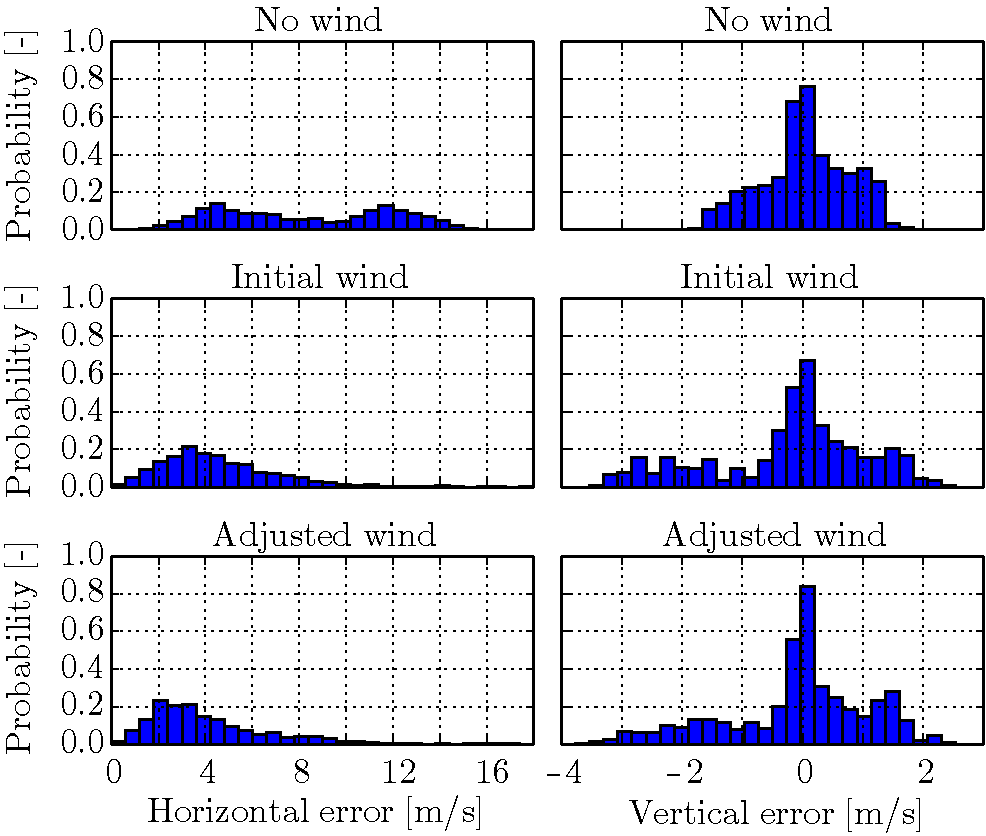
\includegraphics[width=\columnwidth]{images/WindPred/Results/hist_all.pdf}
\caption[Error histograms]{Error histograms: The horizontal error distribution is clearly improved by the downscaling model, but the vertical component is worse than the no wind assumption. }
\label{fig:PL_WindPred_hist_unweighted}
\end{figure}

%%%%%%%%%%%%%%%%%%%%%%%%%%%%%%%%%%%%%%%%%%%%%%%%%%%%%%%%%%%%%%%%%
%%%%%%%%%%%%%%%%%%%%%%%%%%%%%%%%%%%%%%%%%%%%%%%%%%%%%%%%%%%%%%%%%
\section{Conclusion}
\label{sec:PL_WindPred_Conclusion}
%%%%%%%%%%%%%%%%%%%%%%%%%%%%%%%%%%%%%%%%%%%%%%%%%%%%%%%%%%%%%%%%%
%%%%%%%%%%%%%%%%%%%%%%%%%%%%%%%%%%%%%%%%%%%%%%%%%%%%%%%%%%%%%%%%%

This paper has presented the literature's first 3D wind field prediction system designed to run in real-time onboard a UAV. The method is based on downscaling low-resolution wind data from a global weather model via potential flow theory, which guarantees that the terrain boundaries in a high-resolution 2.5D height map, mass conservation and the atmospheric stratification are observed. Due to the model's simplicity, typical flow fields ($\unit[1]{km^3}$ at \unit[25]{m} resolution) are calculated in below \unit[10]{s} on a standard laptop computer. The model yields good qualitative results in synthetic valley and ramp test cases. The comparison to 1D LIDAR profiles collected in the Swiss Alps shows an average horizontal wind error decrease of \unit[41]{\%} over the \emph{zero-wind assumption} that is mostly used in UAV path planning today. However, the vertical wind error is increased by \unit[26]{\%} in contrast to the zero-wind assumption. All in all, as shown in \cref{tab:PL_WindPred_rmse}, the method decreases the overall error with respect to a zero-wind assumption by 23\%. It is thus more accurate than not considering any wind during the planning stage at all, and is also slightly better than the pure interpolation of a global weather model. As a result, path planners can generate safer aircraft trajectories e.g. by avoiding areas of strong horizontal winds. However, due to the simplicity of the model the accuracy is not yet sufficient for the use on fragile or low-power UAVs. Follow-up research is thus required.

\subsection{Future Research}

The remaining uncertainties in this initial evaluation concern the vertical wind error: It is mostly caused by the \emph{Vorab} LIDAR measurements, which contain local anomalies such as mountain waves or thermal flows that are also hard to predict for more sophisticated models and human intuition. The accuracy of the LIDAR data might occasionally be compromised by clouds, fog or precipitation that were not filtered out correctly. To allow a final evaluation of the method's accuracy, more extensive 3D wind field data --- e.g. collected via UAVs with accurate airspeed probes --- therefore needs to be collected in a next step.

However, to reach the vertical wind accuracy required for fragile low-power UAVs, the method itself and its settings also require extensions. Future research is suggested in the following areas: 
\begin{itemize}
\item An increase of the computational domain. This models larger areas of terrain and allows to rudimentarily capture the effect of mountain waves which, as in the \emph{Vorab} test case, may cause significant errors.
\item Online fusion of the wind measurements taken by the UAV along its previous trajectory. This can significantly increase the initial wind field quality. For example, such a method could easily detect and resolve both the wind direction and wind speed errors in $\vec{u}^\text{I}$ in \cref{fig:PL_WindPred_valley_breeze}.
\end{itemize}

If, after implementing those extensions, the current method still does not prove accurate enough, then methods which do not only \emph{adjust} the initial wind field $\vec{u}^\text{I}$, but which completely \emph{recalculate} it will be investigated. Such methods are more complex and closer to \ac{CFD} approaches, and may require machine learning techniques to speed up the calculation.

The feasibility of machine learning techniques to speed up fluid simulations has been shown for example in the fields of computer vision and aerodynamic design. In computer vision \acp{CNN} are used to to speed up fluid simulations by either replacing parts of fluid solvers such as the pressure correction \cite{Tompson2017AEF} or not using a fluid solver at all \cite{Kim2018DeepFluids}. Other approaches use a hybrid LSTM-\ac{CNN} network \cite{Wiewel2018LSP} or a regression forest \cite{Ladicky2015DFS}. The resulting networks speed up the generation of fluid flows up to three orders of magnitudes compared to state-of-the-art fluid solvers. However, those methods developed in computer vision compute how the flow will develop over time and focus on the stability of such a solution instead of the accuracy in the predicted velocity field.

When predicting the wind field over complex terrain only the steady state wind is required and a high velocity accuracy is desired. Umetani and Bickel \cite{Umetani2018LTF} present an machine learning approach for aerdynamic design where they use a Gaussian Progress Regressor to predict the drag coeffienct of an object and the velocity field around it. The \ac{CNN} proposed by Guo et al. \cite{Guo2016CNN} predicts the steady laminar flow around objects and achieve a speed up of up to four order of magnitudes compared to a Lattice Boltzmann Method solver \cite{McNamara1988LBM}. All in all, the presented methods show the feasibility of machine learning methods to replace and speed up current state-of-the-art fluid solvers. However, for accurately predicting the wind over complex terrain the methods still need to be adopted and improved accordingly.

%If sufficient computation time is available, then the time-optimal planner's cost advantage over the shortest-path planner increases with wind speed. However, more important than the optimality of the path is its feasibility: While the wind-aware planner always produces collision-free paths in wind, the shortest path often results in terrain collisions. For safe flight through cluttered terrain and complex wind fields, there is therefore no alternative to using a wind-aware path planner.

\subsection*{Acknowledgements}
We'd like to thank Prof. Bruno Neininger and  David Braig from the Zurich University of Applied Sciences both for providing the LIDAR wind measurements and assistance in evaluating the data.


\bibliographystyle{IEEEtran}
\bibliography{refs/refs_all}

\end{document}
